\documentclass[10pt]{beamer}

\usetheme{metropolis}
\usepackage{tikz}
\usepackage{appendixnumberbeamer}

\usepackage{booktabs}
\usepackage[scale=2]{ccicons}

\usepackage{pgfplots}
\usepgfplotslibrary{dateplot}

\usepackage{xspace}
\newcommand{\themename}{\textbf{\textsc{metropolis}}\xspace}
\usepackage{algorithm}
\usepackage[noend]{algpseudocode}
\usepackage{multimedia}

\makeatletter
\def\BState{\State\hskip-\ALG@thistlm}
\makeatother

\renewcommand{\thealgorithm}{}

 \newcommand{\grille}{
 \begin{tikzpicture}[overlay,remember picture]
   \begin{scope}[shift={(current page.south west)}]
     \draw[gray!50] (0,0) grid[step=2mm] (current page.north east);
     \draw[red!50] (0,0) grid[step=1cm] (current page.north east);
     \draw (0.2,1) node {1};
     \draw (0.2,2) node {2};
     \draw (0.2,3) node {3};
     \draw (0.2,4) node {4};
     \draw (0.2,5) node {5};
     \draw (0.2,6) node {6};
     \draw (0.2,7) node {7};
     \draw (0.2,8) node {8};
     \draw (0.2,9) node {9};
     \draw (1,0.5) node {1};
     \draw (2,0.5) node {2};
     \draw (3,0.5) node {3};
     \draw (4,0.5) node {4};
     \draw (5,0.5) node {5};
     \draw (6,0.5) node {6};
     \draw (7,0.5) node {7};
     \draw (8,0.5) node {8};
     \draw (9,0.5) node {9};
     \draw (10,0.5) node {10};
     \draw (11,0.5) node {11};
     \draw (12,0.5) node {12};
   \end{scope}
 \end{tikzpicture}
 }

\definecolor{mygreen}{RGB}{28,172,0}

\title{\vspace{1cm} A High Performance Implementation of the 2D N-Body Gravitational Problem}
\subtitle{Benchmark of the Barnes-Hut algorithm compared to the Brute-Force algorithm}
\date{June 23, 2016}
\author{Gael Lederrey}
\institute{Parallel and High-Performance Computing - Spring Semester 2016 \\ EPFL-CSE}
\titlegraphic{\includegraphics[height=1.2cm]{./images/EPFL-Logo-CMJN.eps}\hfill\includegraphics[height=1.2cm]{./images/scitas.png}}

\begin{document}

\maketitle

\begin{frame}{Table of contents}
  \setbeamertemplate{section in toc}[sections numbered]
  \tableofcontents[hideallsubsections]
\end{frame}

\section{Project Description}

\begin{frame}{Introduction}

Purpose of this project:
\begin{itemize}
\item Write a fast program to solve a problem
\item Use the knowledge of optimization learned during the course
\item Use MPI to implement a parallel version
\item Compare the theory with the numerical results
\end{itemize}
\onslide<2->
\vspace{0.5cm}
Use-case: 2D N-Body Gravitational problem

\end{frame}

\begin{frame}{N-Body Gravitational problem - Theory}
Gravitational force of body $i$ on body $j$:
\[
\vec{F}_{i\rightarrow j} = G\cdot\frac{m_im_j(\vec{x}_j-\vec{x}_i)}{\Vert \vec{x}_j-\vec{x}_i\Vert^3}
\]
where $G$ is the gravitational constant, $m_i,\,m_j$ are the masses and $\vec{x}_i,\,\vec{x}_j$ are the positions.

\onslide<2->
At each iteration, we will have for body $j$:
\[
\vec{F}_j = \sum_{i=1}^n \vec{F}_{i\rightarrow j}
\]
We can then update it:
\[
\vec{v}_j = \vec{v}_j + \dfrac{dt}{m_j}\cdot \vec{F}_j \qquad \qquad \vec{x}_j = \vec{x}_j + dt\cdot\vec{v}_j
\]

\onslide<3->
\begin{center}
{\bf  How can we compute all the interactions between all the bodies?}
\end{center}

\end{frame}

\begin{frame}{Algorithms}

\begin{itemize}
\onslide<1->
\item {\bf Brute-Force}
\begin{itemize}
\item Compute all the interactions between all the bodies
\item Straight-Forward and easy to implement
\item Complexity: $\mathcal{O}(n^2)$
\end{itemize}
\vspace{0.5cm}
\onslide<2->
\item {\bf Barnes-Hut}
\begin{itemize}
\item Approximation of the far bodies to compute all the forces on a body
\item Not that difficult to implement. (Require more lines of code)
\item Complexity: $\mathcal{O}(n\log n)$
\end{itemize}
\end{itemize}

\end{frame}

\section{Barnes-Hut algorithm in details}

\begin{frame}{General idea}

Idea of this algorithm:
\begin{itemize}
\item Use a precision parameter $\theta$ to approximate the forces of the far bodies using the center of mass
\end{itemize}
\begin{figure}
\centering
\includegraphics[width=0.6\textwidth]{./images/bh.png}
\end{figure}
{\bf How can we do this?} \onslide<2-> $\Rightarrow$ Use a quadtree and the CM of the nodes.
\end{frame}

\begin{frame}{Quadtree}
\only<1>{
\begin{itemize}
\item A quadtree is a tree with four children \\(for the four directions NE, NW, SE and SW)
\item In each leaf, there's a maximum of 1 body. 
\item If a body is added in a leaf with a body, we split the leaf in 4 parts. And we add the two bodies to its children. 
\end{itemize}
}
\only<2-8>{

\begin{tikzpicture}[overlay,remember picture,shift={(current page.south west)}]
%\grille
\draw[line width=1.2] (1,2.3) -- (1,6.3) -- (5,6.3) -- (5,2.3) -- cycle;
\onslide<3->
\draw[fill=black,draw=black] (4.8,2.7) circle (0.1cm);
\node[circle, draw=black, fill=black, scale=0.6]  at (9.4, 7) (A) {};
\only<3-4>{
\node[anchor=east] at (9.3, 7) {1 body};
}
\onslide<4->
\only<4>{
\draw[fill=red,draw=red] (1.7,5.5) circle (0.1cm);
}
\onslide<5->
\only<5-6>{
\node[anchor=east] at (9.3, 7) {2 bodies};
\node[anchor=east] at (7.8, 5) {1 body};
}
\draw[fill=black,draw=black] (1.7,5.5) circle (0.1cm);
\draw[blue] (1,4.3) -- (5,4.3);
\draw[blue] (3,2.3) -- (3,6.3);
\node[circle, draw=black, fill=black, scale=0.6]  at (7.9, 5) (B) {};
\node[circle, draw=black, fill=white, scale=0.6]  at (8.9, 5) (C) {};
\node[circle, draw=black, fill=white, scale=0.6]  at (9.9, 5) (D) {};
\node[circle, draw=black, fill=black, scale=0.6]  at (10.9, 5) (E) {};
\draw[blue] (A)--(B);
\draw[blue] (A)--(C);
\draw[blue] (A)--(D);
\draw[blue] (A)--(E);
\only<6>{
\draw[fill=red,draw=red] (2.5,4.6) circle (0.1cm);
}
\only<7>{
\node[anchor=east] at (9.3, 7) {3 bodies};
\node[anchor=east] at (7.8, 5) {2 bodies};
}
\onslide<7->
\draw[fill=black,draw=black] (2.5,4.6) circle (0.1cm);
\draw[mygreen] (2,4.3) -- (2,6.3);
\draw[mygreen] (1,5.3) -- (3,5.3);
\node[circle, draw=black, fill=black, scale=0.6]  at (7.2, 3) (F) {};
\node[circle, draw=black, fill=white, scale=0.6]  at (7.7, 3) (G) {};
\node[circle, draw=black, fill=white, scale=0.6]  at (8.1, 3) (H) {};
\node[circle, draw=black, fill=black, scale=0.6]  at (8.5, 3) (I) {};
\draw[mygreen] (B)--(F);
\draw[mygreen] (B)--(G);
\draw[mygreen] (B)--(H);
\draw[mygreen] (B)--(I);
\onslide<8->
\only<8>{
\node[anchor=east] at (9.3, 7) {4 bodies};
\node[anchor=east] at (7.8, 5) {2 bodies};
}
\draw[fill=black,draw=black] (4,5) circle (0.1cm);
\draw[fill=black,draw=black] (8.9, 5) circle (0.1cm);
\end{tikzpicture}
}
\only<9>{
\begin{tikzpicture}[overlay,remember picture,shift={(current page.south west)}]
%\grille
\node[anchor=south] at (6,0) {% This file was created by matlab2tikz.
% Minimal pgfplots version: 1.3
%
%The latest updates can be retrieved from
%  http://www.mathworks.com/matlabcentral/fileexchange/22022-matlab2tikz
%where you can also make suggestions and rate matlab2tikz.
%
\begin{tikzpicture}

\begin{axis}[%
width=7cm,
height=7cm,
at={(0.769167in,0.484687in)},
scale only axis,
xmin=-100,
xmax=100,
xlabel={x [AU]},
ymin=-100,
ymax=100,
ylabel={y [AU]},
axis x line*=bottom,
axis y line*=left
]
\addplot [color=blue,solid,forget plot]
  table[row sep=crcr]{%
-100	100\\
100	100\\
};
\addplot [color=blue,solid,forget plot]
  table[row sep=crcr]{%
-100	-100\\
100	-100\\
};
\addplot [color=blue,solid,forget plot]
  table[row sep=crcr]{%
100	-100\\
100	100\\
};
\addplot [color=blue,solid,forget plot]
  table[row sep=crcr]{%
-100	-100\\
-100	100\\
};
\addplot [color=blue,solid,forget plot]
  table[row sep=crcr]{%
0	100\\
100	100\\
};
\addplot [color=blue,solid,forget plot]
  table[row sep=crcr]{%
0	0\\
100	0\\
};
\addplot [color=blue,solid,forget plot]
  table[row sep=crcr]{%
100	0\\
100	100\\
};
\addplot [color=blue,solid,forget plot]
  table[row sep=crcr]{%
0	0\\
0	100\\
};
\addplot [color=blue,solid,forget plot]
  table[row sep=crcr]{%
50	100\\
100	100\\
};
\addplot [color=blue,solid,forget plot]
  table[row sep=crcr]{%
50	50\\
100	50\\
};
\addplot [color=blue,solid,forget plot]
  table[row sep=crcr]{%
100	50\\
100	100\\
};
\addplot [color=blue,solid,forget plot]
  table[row sep=crcr]{%
50	50\\
50	100\\
};
\addplot [color=blue,solid,forget plot]
  table[row sep=crcr]{%
0	100\\
50	100\\
};
\addplot [color=blue,solid,forget plot]
  table[row sep=crcr]{%
0	50\\
50	50\\
};
\addplot [color=blue,solid,forget plot]
  table[row sep=crcr]{%
50	50\\
50	100\\
};
\addplot [color=blue,solid,forget plot]
  table[row sep=crcr]{%
0	50\\
0	100\\
};
\addplot [color=blue,solid,forget plot]
  table[row sep=crcr]{%
25	100\\
50	100\\
};
\addplot [color=blue,solid,forget plot]
  table[row sep=crcr]{%
25	75\\
50	75\\
};
\addplot [color=blue,solid,forget plot]
  table[row sep=crcr]{%
50	75\\
50	100\\
};
\addplot [color=blue,solid,forget plot]
  table[row sep=crcr]{%
25	75\\
25	100\\
};
\addplot [color=blue,solid,forget plot]
  table[row sep=crcr]{%
0	100\\
25	100\\
};
\addplot [color=blue,solid,forget plot]
  table[row sep=crcr]{%
0	75\\
25	75\\
};
\addplot [color=blue,solid,forget plot]
  table[row sep=crcr]{%
25	75\\
25	100\\
};
\addplot [color=blue,solid,forget plot]
  table[row sep=crcr]{%
0	75\\
0	100\\
};
\addplot [color=blue,solid,forget plot]
  table[row sep=crcr]{%
25	75\\
50	75\\
};
\addplot [color=blue,solid,forget plot]
  table[row sep=crcr]{%
25	50\\
50	50\\
};
\addplot [color=blue,solid,forget plot]
  table[row sep=crcr]{%
50	50\\
50	75\\
};
\addplot [color=blue,solid,forget plot]
  table[row sep=crcr]{%
25	50\\
25	75\\
};
\addplot [color=blue,solid,forget plot]
  table[row sep=crcr]{%
37.5	75\\
50	75\\
};
\addplot [color=blue,solid,forget plot]
  table[row sep=crcr]{%
37.5	62.5\\
50	62.5\\
};
\addplot [color=blue,solid,forget plot]
  table[row sep=crcr]{%
50	62.5\\
50	75\\
};
\addplot [color=blue,solid,forget plot]
  table[row sep=crcr]{%
37.5	62.5\\
37.5	75\\
};
\addplot [color=blue,solid,forget plot]
  table[row sep=crcr]{%
25	75\\
37.5	75\\
};
\addplot [color=blue,solid,forget plot]
  table[row sep=crcr]{%
25	62.5\\
37.5	62.5\\
};
\addplot [color=blue,solid,forget plot]
  table[row sep=crcr]{%
37.5	62.5\\
37.5	75\\
};
\addplot [color=blue,solid,forget plot]
  table[row sep=crcr]{%
25	62.5\\
25	75\\
};
\addplot [color=blue,solid,forget plot]
  table[row sep=crcr]{%
37.5	62.5\\
50	62.5\\
};
\addplot [color=blue,solid,forget plot]
  table[row sep=crcr]{%
37.5	50\\
50	50\\
};
\addplot [color=blue,solid,forget plot]
  table[row sep=crcr]{%
50	50\\
50	62.5\\
};
\addplot [color=blue,solid,forget plot]
  table[row sep=crcr]{%
37.5	50\\
37.5	62.5\\
};
\addplot [color=blue,solid,forget plot]
  table[row sep=crcr]{%
25	62.5\\
37.5	62.5\\
};
\addplot [color=blue,solid,forget plot]
  table[row sep=crcr]{%
25	50\\
37.5	50\\
};
\addplot [color=blue,solid,forget plot]
  table[row sep=crcr]{%
37.5	50\\
37.5	62.5\\
};
\addplot [color=blue,solid,forget plot]
  table[row sep=crcr]{%
25	50\\
25	62.5\\
};
\addplot [color=blue,solid,forget plot]
  table[row sep=crcr]{%
0	75\\
25	75\\
};
\addplot [color=blue,solid,forget plot]
  table[row sep=crcr]{%
0	50\\
25	50\\
};
\addplot [color=blue,solid,forget plot]
  table[row sep=crcr]{%
25	50\\
25	75\\
};
\addplot [color=blue,solid,forget plot]
  table[row sep=crcr]{%
0	50\\
0	75\\
};
\addplot [color=blue,solid,forget plot]
  table[row sep=crcr]{%
12.5	75\\
25	75\\
};
\addplot [color=blue,solid,forget plot]
  table[row sep=crcr]{%
12.5	62.5\\
25	62.5\\
};
\addplot [color=blue,solid,forget plot]
  table[row sep=crcr]{%
25	62.5\\
25	75\\
};
\addplot [color=blue,solid,forget plot]
  table[row sep=crcr]{%
12.5	62.5\\
12.5	75\\
};
\addplot [color=blue,solid,forget plot]
  table[row sep=crcr]{%
0	75\\
12.5	75\\
};
\addplot [color=blue,solid,forget plot]
  table[row sep=crcr]{%
0	62.5\\
12.5	62.5\\
};
\addplot [color=blue,solid,forget plot]
  table[row sep=crcr]{%
12.5	62.5\\
12.5	75\\
};
\addplot [color=blue,solid,forget plot]
  table[row sep=crcr]{%
0	62.5\\
0	75\\
};
\addplot [color=blue,solid,forget plot]
  table[row sep=crcr]{%
12.5	62.5\\
25	62.5\\
};
\addplot [color=blue,solid,forget plot]
  table[row sep=crcr]{%
12.5	50\\
25	50\\
};
\addplot [color=blue,solid,forget plot]
  table[row sep=crcr]{%
25	50\\
25	62.5\\
};
\addplot [color=blue,solid,forget plot]
  table[row sep=crcr]{%
12.5	50\\
12.5	62.5\\
};
\addplot [color=blue,solid,forget plot]
  table[row sep=crcr]{%
0	62.5\\
12.5	62.5\\
};
\addplot [color=blue,solid,forget plot]
  table[row sep=crcr]{%
0	50\\
12.5	50\\
};
\addplot [color=blue,solid,forget plot]
  table[row sep=crcr]{%
12.5	50\\
12.5	62.5\\
};
\addplot [color=blue,solid,forget plot]
  table[row sep=crcr]{%
0	50\\
0	62.5\\
};
\addplot [color=blue,solid,forget plot]
  table[row sep=crcr]{%
50	50\\
100	50\\
};
\addplot [color=blue,solid,forget plot]
  table[row sep=crcr]{%
50	0\\
100	0\\
};
\addplot [color=blue,solid,forget plot]
  table[row sep=crcr]{%
100	0\\
100	50\\
};
\addplot [color=blue,solid,forget plot]
  table[row sep=crcr]{%
50	0\\
50	50\\
};
\addplot [color=blue,solid,forget plot]
  table[row sep=crcr]{%
75	50\\
100	50\\
};
\addplot [color=blue,solid,forget plot]
  table[row sep=crcr]{%
75	25\\
100	25\\
};
\addplot [color=blue,solid,forget plot]
  table[row sep=crcr]{%
100	25\\
100	50\\
};
\addplot [color=blue,solid,forget plot]
  table[row sep=crcr]{%
75	25\\
75	50\\
};
\addplot [color=blue,solid,forget plot]
  table[row sep=crcr]{%
50	50\\
75	50\\
};
\addplot [color=blue,solid,forget plot]
  table[row sep=crcr]{%
50	25\\
75	25\\
};
\addplot [color=blue,solid,forget plot]
  table[row sep=crcr]{%
75	25\\
75	50\\
};
\addplot [color=blue,solid,forget plot]
  table[row sep=crcr]{%
50	25\\
50	50\\
};
\addplot [color=blue,solid,forget plot]
  table[row sep=crcr]{%
75	25\\
100	25\\
};
\addplot [color=blue,solid,forget plot]
  table[row sep=crcr]{%
75	0\\
100	0\\
};
\addplot [color=blue,solid,forget plot]
  table[row sep=crcr]{%
100	0\\
100	25\\
};
\addplot [color=blue,solid,forget plot]
  table[row sep=crcr]{%
75	0\\
75	25\\
};
\addplot [color=blue,solid,forget plot]
  table[row sep=crcr]{%
50	25\\
75	25\\
};
\addplot [color=blue,solid,forget plot]
  table[row sep=crcr]{%
50	0\\
75	0\\
};
\addplot [color=blue,solid,forget plot]
  table[row sep=crcr]{%
75	0\\
75	25\\
};
\addplot [color=blue,solid,forget plot]
  table[row sep=crcr]{%
50	0\\
50	25\\
};
\addplot [color=blue,solid,forget plot]
  table[row sep=crcr]{%
62.5	25\\
75	25\\
};
\addplot [color=blue,solid,forget plot]
  table[row sep=crcr]{%
62.5	12.5\\
75	12.5\\
};
\addplot [color=blue,solid,forget plot]
  table[row sep=crcr]{%
75	12.5\\
75	25\\
};
\addplot [color=blue,solid,forget plot]
  table[row sep=crcr]{%
62.5	12.5\\
62.5	25\\
};
\addplot [color=blue,solid,forget plot]
  table[row sep=crcr]{%
50	25\\
62.5	25\\
};
\addplot [color=blue,solid,forget plot]
  table[row sep=crcr]{%
50	12.5\\
62.5	12.5\\
};
\addplot [color=blue,solid,forget plot]
  table[row sep=crcr]{%
62.5	12.5\\
62.5	25\\
};
\addplot [color=blue,solid,forget plot]
  table[row sep=crcr]{%
50	12.5\\
50	25\\
};
\addplot [color=blue,solid,forget plot]
  table[row sep=crcr]{%
56.25	25\\
62.5	25\\
};
\addplot [color=blue,solid,forget plot]
  table[row sep=crcr]{%
56.25	18.75\\
62.5	18.75\\
};
\addplot [color=blue,solid,forget plot]
  table[row sep=crcr]{%
62.5	18.75\\
62.5	25\\
};
\addplot [color=blue,solid,forget plot]
  table[row sep=crcr]{%
56.25	18.75\\
56.25	25\\
};
\addplot [color=blue,solid,forget plot]
  table[row sep=crcr]{%
50	25\\
56.25	25\\
};
\addplot [color=blue,solid,forget plot]
  table[row sep=crcr]{%
50	18.75\\
56.25	18.75\\
};
\addplot [color=blue,solid,forget plot]
  table[row sep=crcr]{%
56.25	18.75\\
56.25	25\\
};
\addplot [color=blue,solid,forget plot]
  table[row sep=crcr]{%
50	18.75\\
50	25\\
};
\addplot [color=blue,solid,forget plot]
  table[row sep=crcr]{%
56.25	18.75\\
62.5	18.75\\
};
\addplot [color=blue,solid,forget plot]
  table[row sep=crcr]{%
56.25	12.5\\
62.5	12.5\\
};
\addplot [color=blue,solid,forget plot]
  table[row sep=crcr]{%
62.5	12.5\\
62.5	18.75\\
};
\addplot [color=blue,solid,forget plot]
  table[row sep=crcr]{%
56.25	12.5\\
56.25	18.75\\
};
\addplot [color=blue,solid,forget plot]
  table[row sep=crcr]{%
50	18.75\\
56.25	18.75\\
};
\addplot [color=blue,solid,forget plot]
  table[row sep=crcr]{%
50	12.5\\
56.25	12.5\\
};
\addplot [color=blue,solid,forget plot]
  table[row sep=crcr]{%
56.25	12.5\\
56.25	18.75\\
};
\addplot [color=blue,solid,forget plot]
  table[row sep=crcr]{%
50	12.5\\
50	18.75\\
};
\addplot [color=blue,solid,forget plot]
  table[row sep=crcr]{%
62.5	12.5\\
75	12.5\\
};
\addplot [color=blue,solid,forget plot]
  table[row sep=crcr]{%
62.5	0\\
75	0\\
};
\addplot [color=blue,solid,forget plot]
  table[row sep=crcr]{%
75	0\\
75	12.5\\
};
\addplot [color=blue,solid,forget plot]
  table[row sep=crcr]{%
62.5	0\\
62.5	12.5\\
};
\addplot [color=blue,solid,forget plot]
  table[row sep=crcr]{%
50	12.5\\
62.5	12.5\\
};
\addplot [color=blue,solid,forget plot]
  table[row sep=crcr]{%
50	0\\
62.5	0\\
};
\addplot [color=blue,solid,forget plot]
  table[row sep=crcr]{%
62.5	0\\
62.5	12.5\\
};
\addplot [color=blue,solid,forget plot]
  table[row sep=crcr]{%
50	0\\
50	12.5\\
};
\addplot [color=blue,solid,forget plot]
  table[row sep=crcr]{%
0	50\\
50	50\\
};
\addplot [color=blue,solid,forget plot]
  table[row sep=crcr]{%
0	0\\
50	0\\
};
\addplot [color=blue,solid,forget plot]
  table[row sep=crcr]{%
50	0\\
50	50\\
};
\addplot [color=blue,solid,forget plot]
  table[row sep=crcr]{%
0	0\\
0	50\\
};
\addplot [color=blue,solid,forget plot]
  table[row sep=crcr]{%
25	50\\
50	50\\
};
\addplot [color=blue,solid,forget plot]
  table[row sep=crcr]{%
25	25\\
50	25\\
};
\addplot [color=blue,solid,forget plot]
  table[row sep=crcr]{%
50	25\\
50	50\\
};
\addplot [color=blue,solid,forget plot]
  table[row sep=crcr]{%
25	25\\
25	50\\
};
\addplot [color=blue,solid,forget plot]
  table[row sep=crcr]{%
37.5	50\\
50	50\\
};
\addplot [color=blue,solid,forget plot]
  table[row sep=crcr]{%
37.5	37.5\\
50	37.5\\
};
\addplot [color=blue,solid,forget plot]
  table[row sep=crcr]{%
50	37.5\\
50	50\\
};
\addplot [color=blue,solid,forget plot]
  table[row sep=crcr]{%
37.5	37.5\\
37.5	50\\
};
\addplot [color=blue,solid,forget plot]
  table[row sep=crcr]{%
43.75	50\\
50	50\\
};
\addplot [color=blue,solid,forget plot]
  table[row sep=crcr]{%
43.75	43.75\\
50	43.75\\
};
\addplot [color=blue,solid,forget plot]
  table[row sep=crcr]{%
50	43.75\\
50	50\\
};
\addplot [color=blue,solid,forget plot]
  table[row sep=crcr]{%
43.75	43.75\\
43.75	50\\
};
\addplot [color=blue,solid,forget plot]
  table[row sep=crcr]{%
37.5	50\\
43.75	50\\
};
\addplot [color=blue,solid,forget plot]
  table[row sep=crcr]{%
37.5	43.75\\
43.75	43.75\\
};
\addplot [color=blue,solid,forget plot]
  table[row sep=crcr]{%
43.75	43.75\\
43.75	50\\
};
\addplot [color=blue,solid,forget plot]
  table[row sep=crcr]{%
37.5	43.75\\
37.5	50\\
};
\addplot [color=blue,solid,forget plot]
  table[row sep=crcr]{%
43.75	43.75\\
50	43.75\\
};
\addplot [color=blue,solid,forget plot]
  table[row sep=crcr]{%
43.75	37.5\\
50	37.5\\
};
\addplot [color=blue,solid,forget plot]
  table[row sep=crcr]{%
50	37.5\\
50	43.75\\
};
\addplot [color=blue,solid,forget plot]
  table[row sep=crcr]{%
43.75	37.5\\
43.75	43.75\\
};
\addplot [color=blue,solid,forget plot]
  table[row sep=crcr]{%
37.5	43.75\\
43.75	43.75\\
};
\addplot [color=blue,solid,forget plot]
  table[row sep=crcr]{%
37.5	37.5\\
43.75	37.5\\
};
\addplot [color=blue,solid,forget plot]
  table[row sep=crcr]{%
43.75	37.5\\
43.75	43.75\\
};
\addplot [color=blue,solid,forget plot]
  table[row sep=crcr]{%
37.5	37.5\\
37.5	43.75\\
};
\addplot [color=blue,solid,forget plot]
  table[row sep=crcr]{%
25	50\\
37.5	50\\
};
\addplot [color=blue,solid,forget plot]
  table[row sep=crcr]{%
25	37.5\\
37.5	37.5\\
};
\addplot [color=blue,solid,forget plot]
  table[row sep=crcr]{%
37.5	37.5\\
37.5	50\\
};
\addplot [color=blue,solid,forget plot]
  table[row sep=crcr]{%
25	37.5\\
25	50\\
};
\addplot [color=blue,solid,forget plot]
  table[row sep=crcr]{%
37.5	37.5\\
50	37.5\\
};
\addplot [color=blue,solid,forget plot]
  table[row sep=crcr]{%
37.5	25\\
50	25\\
};
\addplot [color=blue,solid,forget plot]
  table[row sep=crcr]{%
50	25\\
50	37.5\\
};
\addplot [color=blue,solid,forget plot]
  table[row sep=crcr]{%
37.5	25\\
37.5	37.5\\
};
\addplot [color=blue,solid,forget plot]
  table[row sep=crcr]{%
25	37.5\\
37.5	37.5\\
};
\addplot [color=blue,solid,forget plot]
  table[row sep=crcr]{%
25	25\\
37.5	25\\
};
\addplot [color=blue,solid,forget plot]
  table[row sep=crcr]{%
37.5	25\\
37.5	37.5\\
};
\addplot [color=blue,solid,forget plot]
  table[row sep=crcr]{%
25	25\\
25	37.5\\
};
\addplot [color=blue,solid,forget plot]
  table[row sep=crcr]{%
0	50\\
25	50\\
};
\addplot [color=blue,solid,forget plot]
  table[row sep=crcr]{%
0	25\\
25	25\\
};
\addplot [color=blue,solid,forget plot]
  table[row sep=crcr]{%
25	25\\
25	50\\
};
\addplot [color=blue,solid,forget plot]
  table[row sep=crcr]{%
0	25\\
0	50\\
};
\addplot [color=blue,solid,forget plot]
  table[row sep=crcr]{%
25	25\\
50	25\\
};
\addplot [color=blue,solid,forget plot]
  table[row sep=crcr]{%
25	0\\
50	0\\
};
\addplot [color=blue,solid,forget plot]
  table[row sep=crcr]{%
50	0\\
50	25\\
};
\addplot [color=blue,solid,forget plot]
  table[row sep=crcr]{%
25	0\\
25	25\\
};
\addplot [color=blue,solid,forget plot]
  table[row sep=crcr]{%
37.5	25\\
50	25\\
};
\addplot [color=blue,solid,forget plot]
  table[row sep=crcr]{%
37.5	12.5\\
50	12.5\\
};
\addplot [color=blue,solid,forget plot]
  table[row sep=crcr]{%
50	12.5\\
50	25\\
};
\addplot [color=blue,solid,forget plot]
  table[row sep=crcr]{%
37.5	12.5\\
37.5	25\\
};
\addplot [color=blue,solid,forget plot]
  table[row sep=crcr]{%
25	25\\
37.5	25\\
};
\addplot [color=blue,solid,forget plot]
  table[row sep=crcr]{%
25	12.5\\
37.5	12.5\\
};
\addplot [color=blue,solid,forget plot]
  table[row sep=crcr]{%
37.5	12.5\\
37.5	25\\
};
\addplot [color=blue,solid,forget plot]
  table[row sep=crcr]{%
25	12.5\\
25	25\\
};
\addplot [color=blue,solid,forget plot]
  table[row sep=crcr]{%
37.5	12.5\\
50	12.5\\
};
\addplot [color=blue,solid,forget plot]
  table[row sep=crcr]{%
37.5	0\\
50	0\\
};
\addplot [color=blue,solid,forget plot]
  table[row sep=crcr]{%
50	0\\
50	12.5\\
};
\addplot [color=blue,solid,forget plot]
  table[row sep=crcr]{%
37.5	0\\
37.5	12.5\\
};
\addplot [color=blue,solid,forget plot]
  table[row sep=crcr]{%
43.75	12.5\\
50	12.5\\
};
\addplot [color=blue,solid,forget plot]
  table[row sep=crcr]{%
43.75	6.25\\
50	6.25\\
};
\addplot [color=blue,solid,forget plot]
  table[row sep=crcr]{%
50	6.25\\
50	12.5\\
};
\addplot [color=blue,solid,forget plot]
  table[row sep=crcr]{%
43.75	6.25\\
43.75	12.5\\
};
\addplot [color=blue,solid,forget plot]
  table[row sep=crcr]{%
37.5	12.5\\
43.75	12.5\\
};
\addplot [color=blue,solid,forget plot]
  table[row sep=crcr]{%
37.5	6.25\\
43.75	6.25\\
};
\addplot [color=blue,solid,forget plot]
  table[row sep=crcr]{%
43.75	6.25\\
43.75	12.5\\
};
\addplot [color=blue,solid,forget plot]
  table[row sep=crcr]{%
37.5	6.25\\
37.5	12.5\\
};
\addplot [color=blue,solid,forget plot]
  table[row sep=crcr]{%
43.75	6.25\\
50	6.25\\
};
\addplot [color=blue,solid,forget plot]
  table[row sep=crcr]{%
43.75	0\\
50	0\\
};
\addplot [color=blue,solid,forget plot]
  table[row sep=crcr]{%
50	0\\
50	6.25\\
};
\addplot [color=blue,solid,forget plot]
  table[row sep=crcr]{%
43.75	0\\
43.75	6.25\\
};
\addplot [color=blue,solid,forget plot]
  table[row sep=crcr]{%
37.5	6.25\\
43.75	6.25\\
};
\addplot [color=blue,solid,forget plot]
  table[row sep=crcr]{%
37.5	0\\
43.75	0\\
};
\addplot [color=blue,solid,forget plot]
  table[row sep=crcr]{%
43.75	0\\
43.75	6.25\\
};
\addplot [color=blue,solid,forget plot]
  table[row sep=crcr]{%
37.5	0\\
37.5	6.25\\
};
\addplot [color=blue,solid,forget plot]
  table[row sep=crcr]{%
25	12.5\\
37.5	12.5\\
};
\addplot [color=blue,solid,forget plot]
  table[row sep=crcr]{%
25	0\\
37.5	0\\
};
\addplot [color=blue,solid,forget plot]
  table[row sep=crcr]{%
37.5	0\\
37.5	12.5\\
};
\addplot [color=blue,solid,forget plot]
  table[row sep=crcr]{%
25	0\\
25	12.5\\
};
\addplot [color=blue,solid,forget plot]
  table[row sep=crcr]{%
0	25\\
25	25\\
};
\addplot [color=blue,solid,forget plot]
  table[row sep=crcr]{%
0	0\\
25	0\\
};
\addplot [color=blue,solid,forget plot]
  table[row sep=crcr]{%
25	0\\
25	25\\
};
\addplot [color=blue,solid,forget plot]
  table[row sep=crcr]{%
0	0\\
0	25\\
};
\addplot [color=blue,solid,forget plot]
  table[row sep=crcr]{%
12.5	25\\
25	25\\
};
\addplot [color=blue,solid,forget plot]
  table[row sep=crcr]{%
12.5	12.5\\
25	12.5\\
};
\addplot [color=blue,solid,forget plot]
  table[row sep=crcr]{%
25	12.5\\
25	25\\
};
\addplot [color=blue,solid,forget plot]
  table[row sep=crcr]{%
12.5	12.5\\
12.5	25\\
};
\addplot [color=blue,solid,forget plot]
  table[row sep=crcr]{%
0	25\\
12.5	25\\
};
\addplot [color=blue,solid,forget plot]
  table[row sep=crcr]{%
0	12.5\\
12.5	12.5\\
};
\addplot [color=blue,solid,forget plot]
  table[row sep=crcr]{%
12.5	12.5\\
12.5	25\\
};
\addplot [color=blue,solid,forget plot]
  table[row sep=crcr]{%
0	12.5\\
0	25\\
};
\addplot [color=blue,solid,forget plot]
  table[row sep=crcr]{%
6.25	25\\
12.5	25\\
};
\addplot [color=blue,solid,forget plot]
  table[row sep=crcr]{%
6.25	18.75\\
12.5	18.75\\
};
\addplot [color=blue,solid,forget plot]
  table[row sep=crcr]{%
12.5	18.75\\
12.5	25\\
};
\addplot [color=blue,solid,forget plot]
  table[row sep=crcr]{%
6.25	18.75\\
6.25	25\\
};
\addplot [color=blue,solid,forget plot]
  table[row sep=crcr]{%
0	25\\
6.25	25\\
};
\addplot [color=blue,solid,forget plot]
  table[row sep=crcr]{%
0	18.75\\
6.25	18.75\\
};
\addplot [color=blue,solid,forget plot]
  table[row sep=crcr]{%
6.25	18.75\\
6.25	25\\
};
\addplot [color=blue,solid,forget plot]
  table[row sep=crcr]{%
0	18.75\\
0	25\\
};
\addplot [color=blue,solid,forget plot]
  table[row sep=crcr]{%
6.25	18.75\\
12.5	18.75\\
};
\addplot [color=blue,solid,forget plot]
  table[row sep=crcr]{%
6.25	12.5\\
12.5	12.5\\
};
\addplot [color=blue,solid,forget plot]
  table[row sep=crcr]{%
12.5	12.5\\
12.5	18.75\\
};
\addplot [color=blue,solid,forget plot]
  table[row sep=crcr]{%
6.25	12.5\\
6.25	18.75\\
};
\addplot [color=blue,solid,forget plot]
  table[row sep=crcr]{%
0	18.75\\
6.25	18.75\\
};
\addplot [color=blue,solid,forget plot]
  table[row sep=crcr]{%
0	12.5\\
6.25	12.5\\
};
\addplot [color=blue,solid,forget plot]
  table[row sep=crcr]{%
6.25	12.5\\
6.25	18.75\\
};
\addplot [color=blue,solid,forget plot]
  table[row sep=crcr]{%
0	12.5\\
0	18.75\\
};
\addplot [color=blue,solid,forget plot]
  table[row sep=crcr]{%
12.5	12.5\\
25	12.5\\
};
\addplot [color=blue,solid,forget plot]
  table[row sep=crcr]{%
12.5	0\\
25	0\\
};
\addplot [color=blue,solid,forget plot]
  table[row sep=crcr]{%
25	0\\
25	12.5\\
};
\addplot [color=blue,solid,forget plot]
  table[row sep=crcr]{%
12.5	0\\
12.5	12.5\\
};
\addplot [color=blue,solid,forget plot]
  table[row sep=crcr]{%
0	12.5\\
12.5	12.5\\
};
\addplot [color=blue,solid,forget plot]
  table[row sep=crcr]{%
0	0\\
12.5	0\\
};
\addplot [color=blue,solid,forget plot]
  table[row sep=crcr]{%
12.5	0\\
12.5	12.5\\
};
\addplot [color=blue,solid,forget plot]
  table[row sep=crcr]{%
0	0\\
0	12.5\\
};
\addplot [color=blue,solid,forget plot]
  table[row sep=crcr]{%
-100	100\\
0	100\\
};
\addplot [color=blue,solid,forget plot]
  table[row sep=crcr]{%
-100	0\\
0	0\\
};
\addplot [color=blue,solid,forget plot]
  table[row sep=crcr]{%
0	0\\
0	100\\
};
\addplot [color=blue,solid,forget plot]
  table[row sep=crcr]{%
-100	0\\
-100	100\\
};
\addplot [color=blue,solid,forget plot]
  table[row sep=crcr]{%
-50	100\\
0	100\\
};
\addplot [color=blue,solid,forget plot]
  table[row sep=crcr]{%
-50	50\\
0	50\\
};
\addplot [color=blue,solid,forget plot]
  table[row sep=crcr]{%
0	50\\
0	100\\
};
\addplot [color=blue,solid,forget plot]
  table[row sep=crcr]{%
-50	50\\
-50	100\\
};
\addplot [color=blue,solid,forget plot]
  table[row sep=crcr]{%
-25	100\\
0	100\\
};
\addplot [color=blue,solid,forget plot]
  table[row sep=crcr]{%
-25	75\\
0	75\\
};
\addplot [color=blue,solid,forget plot]
  table[row sep=crcr]{%
0	75\\
0	100\\
};
\addplot [color=blue,solid,forget plot]
  table[row sep=crcr]{%
-25	75\\
-25	100\\
};
\addplot [color=blue,solid,forget plot]
  table[row sep=crcr]{%
-50	100\\
-25	100\\
};
\addplot [color=blue,solid,forget plot]
  table[row sep=crcr]{%
-50	75\\
-25	75\\
};
\addplot [color=blue,solid,forget plot]
  table[row sep=crcr]{%
-25	75\\
-25	100\\
};
\addplot [color=blue,solid,forget plot]
  table[row sep=crcr]{%
-50	75\\
-50	100\\
};
\addplot [color=blue,solid,forget plot]
  table[row sep=crcr]{%
-25	75\\
0	75\\
};
\addplot [color=blue,solid,forget plot]
  table[row sep=crcr]{%
-25	50\\
0	50\\
};
\addplot [color=blue,solid,forget plot]
  table[row sep=crcr]{%
0	50\\
0	75\\
};
\addplot [color=blue,solid,forget plot]
  table[row sep=crcr]{%
-25	50\\
-25	75\\
};
\addplot [color=blue,solid,forget plot]
  table[row sep=crcr]{%
-50	75\\
-25	75\\
};
\addplot [color=blue,solid,forget plot]
  table[row sep=crcr]{%
-50	50\\
-25	50\\
};
\addplot [color=blue,solid,forget plot]
  table[row sep=crcr]{%
-25	50\\
-25	75\\
};
\addplot [color=blue,solid,forget plot]
  table[row sep=crcr]{%
-50	50\\
-50	75\\
};
\addplot [color=blue,solid,forget plot]
  table[row sep=crcr]{%
-37.5	75\\
-25	75\\
};
\addplot [color=blue,solid,forget plot]
  table[row sep=crcr]{%
-37.5	62.5\\
-25	62.5\\
};
\addplot [color=blue,solid,forget plot]
  table[row sep=crcr]{%
-25	62.5\\
-25	75\\
};
\addplot [color=blue,solid,forget plot]
  table[row sep=crcr]{%
-37.5	62.5\\
-37.5	75\\
};
\addplot [color=blue,solid,forget plot]
  table[row sep=crcr]{%
-31.25	75\\
-25	75\\
};
\addplot [color=blue,solid,forget plot]
  table[row sep=crcr]{%
-31.25	68.75\\
-25	68.75\\
};
\addplot [color=blue,solid,forget plot]
  table[row sep=crcr]{%
-25	68.75\\
-25	75\\
};
\addplot [color=blue,solid,forget plot]
  table[row sep=crcr]{%
-31.25	68.75\\
-31.25	75\\
};
\addplot [color=blue,solid,forget plot]
  table[row sep=crcr]{%
-37.5	75\\
-31.25	75\\
};
\addplot [color=blue,solid,forget plot]
  table[row sep=crcr]{%
-37.5	68.75\\
-31.25	68.75\\
};
\addplot [color=blue,solid,forget plot]
  table[row sep=crcr]{%
-31.25	68.75\\
-31.25	75\\
};
\addplot [color=blue,solid,forget plot]
  table[row sep=crcr]{%
-37.5	68.75\\
-37.5	75\\
};
\addplot [color=blue,solid,forget plot]
  table[row sep=crcr]{%
-31.25	68.75\\
-25	68.75\\
};
\addplot [color=blue,solid,forget plot]
  table[row sep=crcr]{%
-31.25	62.5\\
-25	62.5\\
};
\addplot [color=blue,solid,forget plot]
  table[row sep=crcr]{%
-25	62.5\\
-25	68.75\\
};
\addplot [color=blue,solid,forget plot]
  table[row sep=crcr]{%
-31.25	62.5\\
-31.25	68.75\\
};
\addplot [color=blue,solid,forget plot]
  table[row sep=crcr]{%
-37.5	68.75\\
-31.25	68.75\\
};
\addplot [color=blue,solid,forget plot]
  table[row sep=crcr]{%
-37.5	62.5\\
-31.25	62.5\\
};
\addplot [color=blue,solid,forget plot]
  table[row sep=crcr]{%
-31.25	62.5\\
-31.25	68.75\\
};
\addplot [color=blue,solid,forget plot]
  table[row sep=crcr]{%
-37.5	62.5\\
-37.5	68.75\\
};
\addplot [color=blue,solid,forget plot]
  table[row sep=crcr]{%
-34.375	68.75\\
-31.25	68.75\\
};
\addplot [color=blue,solid,forget plot]
  table[row sep=crcr]{%
-34.375	65.625\\
-31.25	65.625\\
};
\addplot [color=blue,solid,forget plot]
  table[row sep=crcr]{%
-31.25	65.625\\
-31.25	68.75\\
};
\addplot [color=blue,solid,forget plot]
  table[row sep=crcr]{%
-34.375	65.625\\
-34.375	68.75\\
};
\addplot [color=blue,solid,forget plot]
  table[row sep=crcr]{%
-37.5	68.75\\
-34.375	68.75\\
};
\addplot [color=blue,solid,forget plot]
  table[row sep=crcr]{%
-37.5	65.625\\
-34.375	65.625\\
};
\addplot [color=blue,solid,forget plot]
  table[row sep=crcr]{%
-34.375	65.625\\
-34.375	68.75\\
};
\addplot [color=blue,solid,forget plot]
  table[row sep=crcr]{%
-37.5	65.625\\
-37.5	68.75\\
};
\addplot [color=blue,solid,forget plot]
  table[row sep=crcr]{%
-34.375	65.625\\
-31.25	65.625\\
};
\addplot [color=blue,solid,forget plot]
  table[row sep=crcr]{%
-34.375	62.5\\
-31.25	62.5\\
};
\addplot [color=blue,solid,forget plot]
  table[row sep=crcr]{%
-31.25	62.5\\
-31.25	65.625\\
};
\addplot [color=blue,solid,forget plot]
  table[row sep=crcr]{%
-34.375	62.5\\
-34.375	65.625\\
};
\addplot [color=blue,solid,forget plot]
  table[row sep=crcr]{%
-32.81245	65.62505\\
-31.24995	65.62505\\
};
\addplot [color=blue,solid,forget plot]
  table[row sep=crcr]{%
-32.81245	64.06255\\
-31.24995	64.06255\\
};
\addplot [color=blue,solid,forget plot]
  table[row sep=crcr]{%
-31.24995	64.06255\\
-31.24995	65.62505\\
};
\addplot [color=blue,solid,forget plot]
  table[row sep=crcr]{%
-32.81245	64.06255\\
-32.81245	65.62505\\
};
\addplot [color=blue,solid,forget plot]
  table[row sep=crcr]{%
-34.37505	65.62505\\
-32.81255	65.62505\\
};
\addplot [color=blue,solid,forget plot]
  table[row sep=crcr]{%
-34.37505	64.06255\\
-32.81255	64.06255\\
};
\addplot [color=blue,solid,forget plot]
  table[row sep=crcr]{%
-32.81255	64.06255\\
-32.81255	65.62505\\
};
\addplot [color=blue,solid,forget plot]
  table[row sep=crcr]{%
-34.37505	64.06255\\
-34.37505	65.62505\\
};
\addplot [color=blue,solid,forget plot]
  table[row sep=crcr]{%
-32.81245	64.06245\\
-31.24995	64.06245\\
};
\addplot [color=blue,solid,forget plot]
  table[row sep=crcr]{%
-32.81245	62.49995\\
-31.24995	62.49995\\
};
\addplot [color=blue,solid,forget plot]
  table[row sep=crcr]{%
-31.24995	62.49995\\
-31.24995	64.06245\\
};
\addplot [color=blue,solid,forget plot]
  table[row sep=crcr]{%
-32.81245	62.49995\\
-32.81245	64.06245\\
};
\addplot [color=blue,solid,forget plot]
  table[row sep=crcr]{%
-34.37505	64.06245\\
-32.81255	64.06245\\
};
\addplot [color=blue,solid,forget plot]
  table[row sep=crcr]{%
-34.37505	62.49995\\
-32.81255	62.49995\\
};
\addplot [color=blue,solid,forget plot]
  table[row sep=crcr]{%
-32.81255	62.49995\\
-32.81255	64.06245\\
};
\addplot [color=blue,solid,forget plot]
  table[row sep=crcr]{%
-34.37505	62.49995\\
-34.37505	64.06245\\
};
\addplot [color=blue,solid,forget plot]
  table[row sep=crcr]{%
-37.5	65.625\\
-34.375	65.625\\
};
\addplot [color=blue,solid,forget plot]
  table[row sep=crcr]{%
-37.5	62.5\\
-34.375	62.5\\
};
\addplot [color=blue,solid,forget plot]
  table[row sep=crcr]{%
-34.375	62.5\\
-34.375	65.625\\
};
\addplot [color=blue,solid,forget plot]
  table[row sep=crcr]{%
-37.5	62.5\\
-37.5	65.625\\
};
\addplot [color=blue,solid,forget plot]
  table[row sep=crcr]{%
-50	75\\
-37.5	75\\
};
\addplot [color=blue,solid,forget plot]
  table[row sep=crcr]{%
-50	62.5\\
-37.5	62.5\\
};
\addplot [color=blue,solid,forget plot]
  table[row sep=crcr]{%
-37.5	62.5\\
-37.5	75\\
};
\addplot [color=blue,solid,forget plot]
  table[row sep=crcr]{%
-50	62.5\\
-50	75\\
};
\addplot [color=blue,solid,forget plot]
  table[row sep=crcr]{%
-37.5	62.5\\
-25	62.5\\
};
\addplot [color=blue,solid,forget plot]
  table[row sep=crcr]{%
-37.5	50\\
-25	50\\
};
\addplot [color=blue,solid,forget plot]
  table[row sep=crcr]{%
-25	50\\
-25	62.5\\
};
\addplot [color=blue,solid,forget plot]
  table[row sep=crcr]{%
-37.5	50\\
-37.5	62.5\\
};
\addplot [color=blue,solid,forget plot]
  table[row sep=crcr]{%
-50	62.5\\
-37.5	62.5\\
};
\addplot [color=blue,solid,forget plot]
  table[row sep=crcr]{%
-50	50\\
-37.5	50\\
};
\addplot [color=blue,solid,forget plot]
  table[row sep=crcr]{%
-37.5	50\\
-37.5	62.5\\
};
\addplot [color=blue,solid,forget plot]
  table[row sep=crcr]{%
-50	50\\
-50	62.5\\
};
\addplot [color=blue,solid,forget plot]
  table[row sep=crcr]{%
-43.75	62.5\\
-37.5	62.5\\
};
\addplot [color=blue,solid,forget plot]
  table[row sep=crcr]{%
-43.75	56.25\\
-37.5	56.25\\
};
\addplot [color=blue,solid,forget plot]
  table[row sep=crcr]{%
-37.5	56.25\\
-37.5	62.5\\
};
\addplot [color=blue,solid,forget plot]
  table[row sep=crcr]{%
-43.75	56.25\\
-43.75	62.5\\
};
\addplot [color=blue,solid,forget plot]
  table[row sep=crcr]{%
-50	62.5\\
-43.75	62.5\\
};
\addplot [color=blue,solid,forget plot]
  table[row sep=crcr]{%
-50	56.25\\
-43.75	56.25\\
};
\addplot [color=blue,solid,forget plot]
  table[row sep=crcr]{%
-43.75	56.25\\
-43.75	62.5\\
};
\addplot [color=blue,solid,forget plot]
  table[row sep=crcr]{%
-50	56.25\\
-50	62.5\\
};
\addplot [color=blue,solid,forget plot]
  table[row sep=crcr]{%
-43.75	56.25\\
-37.5	56.25\\
};
\addplot [color=blue,solid,forget plot]
  table[row sep=crcr]{%
-43.75	50\\
-37.5	50\\
};
\addplot [color=blue,solid,forget plot]
  table[row sep=crcr]{%
-37.5	50\\
-37.5	56.25\\
};
\addplot [color=blue,solid,forget plot]
  table[row sep=crcr]{%
-43.75	50\\
-43.75	56.25\\
};
\addplot [color=blue,solid,forget plot]
  table[row sep=crcr]{%
-50	56.25\\
-43.75	56.25\\
};
\addplot [color=blue,solid,forget plot]
  table[row sep=crcr]{%
-50	50\\
-43.75	50\\
};
\addplot [color=blue,solid,forget plot]
  table[row sep=crcr]{%
-43.75	50\\
-43.75	56.25\\
};
\addplot [color=blue,solid,forget plot]
  table[row sep=crcr]{%
-50	50\\
-50	56.25\\
};
\addplot [color=blue,solid,forget plot]
  table[row sep=crcr]{%
-100	100\\
-50	100\\
};
\addplot [color=blue,solid,forget plot]
  table[row sep=crcr]{%
-100	50\\
-50	50\\
};
\addplot [color=blue,solid,forget plot]
  table[row sep=crcr]{%
-50	50\\
-50	100\\
};
\addplot [color=blue,solid,forget plot]
  table[row sep=crcr]{%
-100	50\\
-100	100\\
};
\addplot [color=blue,solid,forget plot]
  table[row sep=crcr]{%
-75	100\\
-50	100\\
};
\addplot [color=blue,solid,forget plot]
  table[row sep=crcr]{%
-75	75\\
-50	75\\
};
\addplot [color=blue,solid,forget plot]
  table[row sep=crcr]{%
-50	75\\
-50	100\\
};
\addplot [color=blue,solid,forget plot]
  table[row sep=crcr]{%
-75	75\\
-75	100\\
};
\addplot [color=blue,solid,forget plot]
  table[row sep=crcr]{%
-100	100\\
-75	100\\
};
\addplot [color=blue,solid,forget plot]
  table[row sep=crcr]{%
-100	75\\
-75	75\\
};
\addplot [color=blue,solid,forget plot]
  table[row sep=crcr]{%
-75	75\\
-75	100\\
};
\addplot [color=blue,solid,forget plot]
  table[row sep=crcr]{%
-100	75\\
-100	100\\
};
\addplot [color=blue,solid,forget plot]
  table[row sep=crcr]{%
-75	75\\
-50	75\\
};
\addplot [color=blue,solid,forget plot]
  table[row sep=crcr]{%
-75	50\\
-50	50\\
};
\addplot [color=blue,solid,forget plot]
  table[row sep=crcr]{%
-50	50\\
-50	75\\
};
\addplot [color=blue,solid,forget plot]
  table[row sep=crcr]{%
-75	50\\
-75	75\\
};
\addplot [color=blue,solid,forget plot]
  table[row sep=crcr]{%
-62.5	75\\
-50	75\\
};
\addplot [color=blue,solid,forget plot]
  table[row sep=crcr]{%
-62.5	62.5\\
-50	62.5\\
};
\addplot [color=blue,solid,forget plot]
  table[row sep=crcr]{%
-50	62.5\\
-50	75\\
};
\addplot [color=blue,solid,forget plot]
  table[row sep=crcr]{%
-62.5	62.5\\
-62.5	75\\
};
\addplot [color=blue,solid,forget plot]
  table[row sep=crcr]{%
-75	75\\
-62.5	75\\
};
\addplot [color=blue,solid,forget plot]
  table[row sep=crcr]{%
-75	62.5\\
-62.5	62.5\\
};
\addplot [color=blue,solid,forget plot]
  table[row sep=crcr]{%
-62.5	62.5\\
-62.5	75\\
};
\addplot [color=blue,solid,forget plot]
  table[row sep=crcr]{%
-75	62.5\\
-75	75\\
};
\addplot [color=blue,solid,forget plot]
  table[row sep=crcr]{%
-68.75	75\\
-62.5	75\\
};
\addplot [color=blue,solid,forget plot]
  table[row sep=crcr]{%
-68.75	68.75\\
-62.5	68.75\\
};
\addplot [color=blue,solid,forget plot]
  table[row sep=crcr]{%
-62.5	68.75\\
-62.5	75\\
};
\addplot [color=blue,solid,forget plot]
  table[row sep=crcr]{%
-68.75	68.75\\
-68.75	75\\
};
\addplot [color=blue,solid,forget plot]
  table[row sep=crcr]{%
-75	75\\
-68.75	75\\
};
\addplot [color=blue,solid,forget plot]
  table[row sep=crcr]{%
-75	68.75\\
-68.75	68.75\\
};
\addplot [color=blue,solid,forget plot]
  table[row sep=crcr]{%
-68.75	68.75\\
-68.75	75\\
};
\addplot [color=blue,solid,forget plot]
  table[row sep=crcr]{%
-75	68.75\\
-75	75\\
};
\addplot [color=blue,solid,forget plot]
  table[row sep=crcr]{%
-68.75	68.75\\
-62.5	68.75\\
};
\addplot [color=blue,solid,forget plot]
  table[row sep=crcr]{%
-68.75	62.5\\
-62.5	62.5\\
};
\addplot [color=blue,solid,forget plot]
  table[row sep=crcr]{%
-62.5	62.5\\
-62.5	68.75\\
};
\addplot [color=blue,solid,forget plot]
  table[row sep=crcr]{%
-68.75	62.5\\
-68.75	68.75\\
};
\addplot [color=blue,solid,forget plot]
  table[row sep=crcr]{%
-75	68.75\\
-68.75	68.75\\
};
\addplot [color=blue,solid,forget plot]
  table[row sep=crcr]{%
-75	62.5\\
-68.75	62.5\\
};
\addplot [color=blue,solid,forget plot]
  table[row sep=crcr]{%
-68.75	62.5\\
-68.75	68.75\\
};
\addplot [color=blue,solid,forget plot]
  table[row sep=crcr]{%
-75	62.5\\
-75	68.75\\
};
\addplot [color=blue,solid,forget plot]
  table[row sep=crcr]{%
-62.5	62.5\\
-50	62.5\\
};
\addplot [color=blue,solid,forget plot]
  table[row sep=crcr]{%
-62.5	50\\
-50	50\\
};
\addplot [color=blue,solid,forget plot]
  table[row sep=crcr]{%
-50	50\\
-50	62.5\\
};
\addplot [color=blue,solid,forget plot]
  table[row sep=crcr]{%
-62.5	50\\
-62.5	62.5\\
};
\addplot [color=blue,solid,forget plot]
  table[row sep=crcr]{%
-75	62.5\\
-62.5	62.5\\
};
\addplot [color=blue,solid,forget plot]
  table[row sep=crcr]{%
-75	50\\
-62.5	50\\
};
\addplot [color=blue,solid,forget plot]
  table[row sep=crcr]{%
-62.5	50\\
-62.5	62.5\\
};
\addplot [color=blue,solid,forget plot]
  table[row sep=crcr]{%
-75	50\\
-75	62.5\\
};
\addplot [color=blue,solid,forget plot]
  table[row sep=crcr]{%
-100	75\\
-75	75\\
};
\addplot [color=blue,solid,forget plot]
  table[row sep=crcr]{%
-100	50\\
-75	50\\
};
\addplot [color=blue,solid,forget plot]
  table[row sep=crcr]{%
-75	50\\
-75	75\\
};
\addplot [color=blue,solid,forget plot]
  table[row sep=crcr]{%
-100	50\\
-100	75\\
};
\addplot [color=blue,solid,forget plot]
  table[row sep=crcr]{%
-87.5	75\\
-75	75\\
};
\addplot [color=blue,solid,forget plot]
  table[row sep=crcr]{%
-87.5	62.5\\
-75	62.5\\
};
\addplot [color=blue,solid,forget plot]
  table[row sep=crcr]{%
-75	62.5\\
-75	75\\
};
\addplot [color=blue,solid,forget plot]
  table[row sep=crcr]{%
-87.5	62.5\\
-87.5	75\\
};
\addplot [color=blue,solid,forget plot]
  table[row sep=crcr]{%
-100	75\\
-87.5	75\\
};
\addplot [color=blue,solid,forget plot]
  table[row sep=crcr]{%
-100	62.5\\
-87.5	62.5\\
};
\addplot [color=blue,solid,forget plot]
  table[row sep=crcr]{%
-87.5	62.5\\
-87.5	75\\
};
\addplot [color=blue,solid,forget plot]
  table[row sep=crcr]{%
-100	62.5\\
-100	75\\
};
\addplot [color=blue,solid,forget plot]
  table[row sep=crcr]{%
-87.5	62.5\\
-75	62.5\\
};
\addplot [color=blue,solid,forget plot]
  table[row sep=crcr]{%
-87.5	50\\
-75	50\\
};
\addplot [color=blue,solid,forget plot]
  table[row sep=crcr]{%
-75	50\\
-75	62.5\\
};
\addplot [color=blue,solid,forget plot]
  table[row sep=crcr]{%
-87.5	50\\
-87.5	62.5\\
};
\addplot [color=blue,solid,forget plot]
  table[row sep=crcr]{%
-81.25	62.5\\
-75	62.5\\
};
\addplot [color=blue,solid,forget plot]
  table[row sep=crcr]{%
-81.25	56.25\\
-75	56.25\\
};
\addplot [color=blue,solid,forget plot]
  table[row sep=crcr]{%
-75	56.25\\
-75	62.5\\
};
\addplot [color=blue,solid,forget plot]
  table[row sep=crcr]{%
-81.25	56.25\\
-81.25	62.5\\
};
\addplot [color=blue,solid,forget plot]
  table[row sep=crcr]{%
-87.5	62.5\\
-81.25	62.5\\
};
\addplot [color=blue,solid,forget plot]
  table[row sep=crcr]{%
-87.5	56.25\\
-81.25	56.25\\
};
\addplot [color=blue,solid,forget plot]
  table[row sep=crcr]{%
-81.25	56.25\\
-81.25	62.5\\
};
\addplot [color=blue,solid,forget plot]
  table[row sep=crcr]{%
-87.5	56.25\\
-87.5	62.5\\
};
\addplot [color=blue,solid,forget plot]
  table[row sep=crcr]{%
-81.25	56.25\\
-75	56.25\\
};
\addplot [color=blue,solid,forget plot]
  table[row sep=crcr]{%
-81.25	50\\
-75	50\\
};
\addplot [color=blue,solid,forget plot]
  table[row sep=crcr]{%
-75	50\\
-75	56.25\\
};
\addplot [color=blue,solid,forget plot]
  table[row sep=crcr]{%
-81.25	50\\
-81.25	56.25\\
};
\addplot [color=blue,solid,forget plot]
  table[row sep=crcr]{%
-87.5	56.25\\
-81.25	56.25\\
};
\addplot [color=blue,solid,forget plot]
  table[row sep=crcr]{%
-87.5	50\\
-81.25	50\\
};
\addplot [color=blue,solid,forget plot]
  table[row sep=crcr]{%
-81.25	50\\
-81.25	56.25\\
};
\addplot [color=blue,solid,forget plot]
  table[row sep=crcr]{%
-87.5	50\\
-87.5	56.25\\
};
\addplot [color=blue,solid,forget plot]
  table[row sep=crcr]{%
-100	62.5\\
-87.5	62.5\\
};
\addplot [color=blue,solid,forget plot]
  table[row sep=crcr]{%
-100	50\\
-87.5	50\\
};
\addplot [color=blue,solid,forget plot]
  table[row sep=crcr]{%
-87.5	50\\
-87.5	62.5\\
};
\addplot [color=blue,solid,forget plot]
  table[row sep=crcr]{%
-100	50\\
-100	62.5\\
};
\addplot [color=blue,solid,forget plot]
  table[row sep=crcr]{%
-50	50\\
0	50\\
};
\addplot [color=blue,solid,forget plot]
  table[row sep=crcr]{%
-50	0\\
0	0\\
};
\addplot [color=blue,solid,forget plot]
  table[row sep=crcr]{%
0	0\\
0	50\\
};
\addplot [color=blue,solid,forget plot]
  table[row sep=crcr]{%
-50	0\\
-50	50\\
};
\addplot [color=blue,solid,forget plot]
  table[row sep=crcr]{%
-25	50\\
0	50\\
};
\addplot [color=blue,solid,forget plot]
  table[row sep=crcr]{%
-25	25\\
0	25\\
};
\addplot [color=blue,solid,forget plot]
  table[row sep=crcr]{%
0	25\\
0	50\\
};
\addplot [color=blue,solid,forget plot]
  table[row sep=crcr]{%
-25	25\\
-25	50\\
};
\addplot [color=blue,solid,forget plot]
  table[row sep=crcr]{%
-12.5	50\\
0	50\\
};
\addplot [color=blue,solid,forget plot]
  table[row sep=crcr]{%
-12.5	37.5\\
0	37.5\\
};
\addplot [color=blue,solid,forget plot]
  table[row sep=crcr]{%
0	37.5\\
0	50\\
};
\addplot [color=blue,solid,forget plot]
  table[row sep=crcr]{%
-12.5	37.5\\
-12.5	50\\
};
\addplot [color=blue,solid,forget plot]
  table[row sep=crcr]{%
-25	50\\
-12.5	50\\
};
\addplot [color=blue,solid,forget plot]
  table[row sep=crcr]{%
-25	37.5\\
-12.5	37.5\\
};
\addplot [color=blue,solid,forget plot]
  table[row sep=crcr]{%
-12.5	37.5\\
-12.5	50\\
};
\addplot [color=blue,solid,forget plot]
  table[row sep=crcr]{%
-25	37.5\\
-25	50\\
};
\addplot [color=blue,solid,forget plot]
  table[row sep=crcr]{%
-12.5	37.5\\
0	37.5\\
};
\addplot [color=blue,solid,forget plot]
  table[row sep=crcr]{%
-12.5	25\\
0	25\\
};
\addplot [color=blue,solid,forget plot]
  table[row sep=crcr]{%
0	25\\
0	37.5\\
};
\addplot [color=blue,solid,forget plot]
  table[row sep=crcr]{%
-12.5	25\\
-12.5	37.5\\
};
\addplot [color=blue,solid,forget plot]
  table[row sep=crcr]{%
-25	37.5\\
-12.5	37.5\\
};
\addplot [color=blue,solid,forget plot]
  table[row sep=crcr]{%
-25	25\\
-12.5	25\\
};
\addplot [color=blue,solid,forget plot]
  table[row sep=crcr]{%
-12.5	25\\
-12.5	37.5\\
};
\addplot [color=blue,solid,forget plot]
  table[row sep=crcr]{%
-25	25\\
-25	37.5\\
};
\addplot [color=blue,solid,forget plot]
  table[row sep=crcr]{%
-50	50\\
-25	50\\
};
\addplot [color=blue,solid,forget plot]
  table[row sep=crcr]{%
-50	25\\
-25	25\\
};
\addplot [color=blue,solid,forget plot]
  table[row sep=crcr]{%
-25	25\\
-25	50\\
};
\addplot [color=blue,solid,forget plot]
  table[row sep=crcr]{%
-50	25\\
-50	50\\
};
\addplot [color=blue,solid,forget plot]
  table[row sep=crcr]{%
-37.5	50\\
-25	50\\
};
\addplot [color=blue,solid,forget plot]
  table[row sep=crcr]{%
-37.5	37.5\\
-25	37.5\\
};
\addplot [color=blue,solid,forget plot]
  table[row sep=crcr]{%
-25	37.5\\
-25	50\\
};
\addplot [color=blue,solid,forget plot]
  table[row sep=crcr]{%
-37.5	37.5\\
-37.5	50\\
};
\addplot [color=blue,solid,forget plot]
  table[row sep=crcr]{%
-50	50\\
-37.5	50\\
};
\addplot [color=blue,solid,forget plot]
  table[row sep=crcr]{%
-50	37.5\\
-37.5	37.5\\
};
\addplot [color=blue,solid,forget plot]
  table[row sep=crcr]{%
-37.5	37.5\\
-37.5	50\\
};
\addplot [color=blue,solid,forget plot]
  table[row sep=crcr]{%
-50	37.5\\
-50	50\\
};
\addplot [color=blue,solid,forget plot]
  table[row sep=crcr]{%
-37.5	37.5\\
-25	37.5\\
};
\addplot [color=blue,solid,forget plot]
  table[row sep=crcr]{%
-37.5	25\\
-25	25\\
};
\addplot [color=blue,solid,forget plot]
  table[row sep=crcr]{%
-25	25\\
-25	37.5\\
};
\addplot [color=blue,solid,forget plot]
  table[row sep=crcr]{%
-37.5	25\\
-37.5	37.5\\
};
\addplot [color=blue,solid,forget plot]
  table[row sep=crcr]{%
-50	37.5\\
-37.5	37.5\\
};
\addplot [color=blue,solid,forget plot]
  table[row sep=crcr]{%
-50	25\\
-37.5	25\\
};
\addplot [color=blue,solid,forget plot]
  table[row sep=crcr]{%
-37.5	25\\
-37.5	37.5\\
};
\addplot [color=blue,solid,forget plot]
  table[row sep=crcr]{%
-50	25\\
-50	37.5\\
};
\addplot [color=blue,solid,forget plot]
  table[row sep=crcr]{%
-25	25\\
0	25\\
};
\addplot [color=blue,solid,forget plot]
  table[row sep=crcr]{%
-25	0\\
0	0\\
};
\addplot [color=blue,solid,forget plot]
  table[row sep=crcr]{%
0	0\\
0	25\\
};
\addplot [color=blue,solid,forget plot]
  table[row sep=crcr]{%
-25	0\\
-25	25\\
};
\addplot [color=blue,solid,forget plot]
  table[row sep=crcr]{%
-50	25\\
-25	25\\
};
\addplot [color=blue,solid,forget plot]
  table[row sep=crcr]{%
-50	0\\
-25	0\\
};
\addplot [color=blue,solid,forget plot]
  table[row sep=crcr]{%
-25	0\\
-25	25\\
};
\addplot [color=blue,solid,forget plot]
  table[row sep=crcr]{%
-50	0\\
-50	25\\
};
\addplot [color=blue,solid,forget plot]
  table[row sep=crcr]{%
-37.5	25\\
-25	25\\
};
\addplot [color=blue,solid,forget plot]
  table[row sep=crcr]{%
-37.5	12.5\\
-25	12.5\\
};
\addplot [color=blue,solid,forget plot]
  table[row sep=crcr]{%
-25	12.5\\
-25	25\\
};
\addplot [color=blue,solid,forget plot]
  table[row sep=crcr]{%
-37.5	12.5\\
-37.5	25\\
};
\addplot [color=blue,solid,forget plot]
  table[row sep=crcr]{%
-50	25\\
-37.5	25\\
};
\addplot [color=blue,solid,forget plot]
  table[row sep=crcr]{%
-50	12.5\\
-37.5	12.5\\
};
\addplot [color=blue,solid,forget plot]
  table[row sep=crcr]{%
-37.5	12.5\\
-37.5	25\\
};
\addplot [color=blue,solid,forget plot]
  table[row sep=crcr]{%
-50	12.5\\
-50	25\\
};
\addplot [color=blue,solid,forget plot]
  table[row sep=crcr]{%
-37.5	12.5\\
-25	12.5\\
};
\addplot [color=blue,solid,forget plot]
  table[row sep=crcr]{%
-37.5	0\\
-25	0\\
};
\addplot [color=blue,solid,forget plot]
  table[row sep=crcr]{%
-25	0\\
-25	12.5\\
};
\addplot [color=blue,solid,forget plot]
  table[row sep=crcr]{%
-37.5	0\\
-37.5	12.5\\
};
\addplot [color=blue,solid,forget plot]
  table[row sep=crcr]{%
-50	12.5\\
-37.5	12.5\\
};
\addplot [color=blue,solid,forget plot]
  table[row sep=crcr]{%
-50	0\\
-37.5	0\\
};
\addplot [color=blue,solid,forget plot]
  table[row sep=crcr]{%
-37.5	0\\
-37.5	12.5\\
};
\addplot [color=blue,solid,forget plot]
  table[row sep=crcr]{%
-50	0\\
-50	12.5\\
};
\addplot [color=blue,solid,forget plot]
  table[row sep=crcr]{%
-100	50\\
-50	50\\
};
\addplot [color=blue,solid,forget plot]
  table[row sep=crcr]{%
-100	0\\
-50	0\\
};
\addplot [color=blue,solid,forget plot]
  table[row sep=crcr]{%
-50	0\\
-50	50\\
};
\addplot [color=blue,solid,forget plot]
  table[row sep=crcr]{%
-100	0\\
-100	50\\
};
\addplot [color=blue,solid,forget plot]
  table[row sep=crcr]{%
-75	50\\
-50	50\\
};
\addplot [color=blue,solid,forget plot]
  table[row sep=crcr]{%
-75	25\\
-50	25\\
};
\addplot [color=blue,solid,forget plot]
  table[row sep=crcr]{%
-50	25\\
-50	50\\
};
\addplot [color=blue,solid,forget plot]
  table[row sep=crcr]{%
-75	25\\
-75	50\\
};
\addplot [color=blue,solid,forget plot]
  table[row sep=crcr]{%
-62.5	50\\
-50	50\\
};
\addplot [color=blue,solid,forget plot]
  table[row sep=crcr]{%
-62.5	37.5\\
-50	37.5\\
};
\addplot [color=blue,solid,forget plot]
  table[row sep=crcr]{%
-50	37.5\\
-50	50\\
};
\addplot [color=blue,solid,forget plot]
  table[row sep=crcr]{%
-62.5	37.5\\
-62.5	50\\
};
\addplot [color=blue,solid,forget plot]
  table[row sep=crcr]{%
-75	50\\
-62.5	50\\
};
\addplot [color=blue,solid,forget plot]
  table[row sep=crcr]{%
-75	37.5\\
-62.5	37.5\\
};
\addplot [color=blue,solid,forget plot]
  table[row sep=crcr]{%
-62.5	37.5\\
-62.5	50\\
};
\addplot [color=blue,solid,forget plot]
  table[row sep=crcr]{%
-75	37.5\\
-75	50\\
};
\addplot [color=blue,solid,forget plot]
  table[row sep=crcr]{%
-62.5	37.5\\
-50	37.5\\
};
\addplot [color=blue,solid,forget plot]
  table[row sep=crcr]{%
-62.5	25\\
-50	25\\
};
\addplot [color=blue,solid,forget plot]
  table[row sep=crcr]{%
-50	25\\
-50	37.5\\
};
\addplot [color=blue,solid,forget plot]
  table[row sep=crcr]{%
-62.5	25\\
-62.5	37.5\\
};
\addplot [color=blue,solid,forget plot]
  table[row sep=crcr]{%
-75	37.5\\
-62.5	37.5\\
};
\addplot [color=blue,solid,forget plot]
  table[row sep=crcr]{%
-75	25\\
-62.5	25\\
};
\addplot [color=blue,solid,forget plot]
  table[row sep=crcr]{%
-62.5	25\\
-62.5	37.5\\
};
\addplot [color=blue,solid,forget plot]
  table[row sep=crcr]{%
-75	25\\
-75	37.5\\
};
\addplot [color=blue,solid,forget plot]
  table[row sep=crcr]{%
-100	50\\
-75	50\\
};
\addplot [color=blue,solid,forget plot]
  table[row sep=crcr]{%
-100	25\\
-75	25\\
};
\addplot [color=blue,solid,forget plot]
  table[row sep=crcr]{%
-75	25\\
-75	50\\
};
\addplot [color=blue,solid,forget plot]
  table[row sep=crcr]{%
-100	25\\
-100	50\\
};
\addplot [color=blue,solid,forget plot]
  table[row sep=crcr]{%
-75	25\\
-50	25\\
};
\addplot [color=blue,solid,forget plot]
  table[row sep=crcr]{%
-75	0\\
-50	0\\
};
\addplot [color=blue,solid,forget plot]
  table[row sep=crcr]{%
-50	0\\
-50	25\\
};
\addplot [color=blue,solid,forget plot]
  table[row sep=crcr]{%
-75	0\\
-75	25\\
};
\addplot [color=blue,solid,forget plot]
  table[row sep=crcr]{%
-62.5	25\\
-50	25\\
};
\addplot [color=blue,solid,forget plot]
  table[row sep=crcr]{%
-62.5	12.5\\
-50	12.5\\
};
\addplot [color=blue,solid,forget plot]
  table[row sep=crcr]{%
-50	12.5\\
-50	25\\
};
\addplot [color=blue,solid,forget plot]
  table[row sep=crcr]{%
-62.5	12.5\\
-62.5	25\\
};
\addplot [color=blue,solid,forget plot]
  table[row sep=crcr]{%
-75	25\\
-62.5	25\\
};
\addplot [color=blue,solid,forget plot]
  table[row sep=crcr]{%
-75	12.5\\
-62.5	12.5\\
};
\addplot [color=blue,solid,forget plot]
  table[row sep=crcr]{%
-62.5	12.5\\
-62.5	25\\
};
\addplot [color=blue,solid,forget plot]
  table[row sep=crcr]{%
-75	12.5\\
-75	25\\
};
\addplot [color=blue,solid,forget plot]
  table[row sep=crcr]{%
-62.5	12.5\\
-50	12.5\\
};
\addplot [color=blue,solid,forget plot]
  table[row sep=crcr]{%
-62.5	0\\
-50	0\\
};
\addplot [color=blue,solid,forget plot]
  table[row sep=crcr]{%
-50	0\\
-50	12.5\\
};
\addplot [color=blue,solid,forget plot]
  table[row sep=crcr]{%
-62.5	0\\
-62.5	12.5\\
};
\addplot [color=blue,solid,forget plot]
  table[row sep=crcr]{%
-75	12.5\\
-62.5	12.5\\
};
\addplot [color=blue,solid,forget plot]
  table[row sep=crcr]{%
-75	0\\
-62.5	0\\
};
\addplot [color=blue,solid,forget plot]
  table[row sep=crcr]{%
-62.5	0\\
-62.5	12.5\\
};
\addplot [color=blue,solid,forget plot]
  table[row sep=crcr]{%
-75	0\\
-75	12.5\\
};
\addplot [color=blue,solid,forget plot]
  table[row sep=crcr]{%
-100	25\\
-75	25\\
};
\addplot [color=blue,solid,forget plot]
  table[row sep=crcr]{%
-100	0\\
-75	0\\
};
\addplot [color=blue,solid,forget plot]
  table[row sep=crcr]{%
-75	0\\
-75	25\\
};
\addplot [color=blue,solid,forget plot]
  table[row sep=crcr]{%
-100	0\\
-100	25\\
};
\addplot [color=blue,solid,forget plot]
  table[row sep=crcr]{%
0	0\\
100	0\\
};
\addplot [color=blue,solid,forget plot]
  table[row sep=crcr]{%
0	-100\\
100	-100\\
};
\addplot [color=blue,solid,forget plot]
  table[row sep=crcr]{%
100	-100\\
100	0\\
};
\addplot [color=blue,solid,forget plot]
  table[row sep=crcr]{%
0	-100\\
0	0\\
};
\addplot [color=blue,solid,forget plot]
  table[row sep=crcr]{%
50	0\\
100	0\\
};
\addplot [color=blue,solid,forget plot]
  table[row sep=crcr]{%
50	-50\\
100	-50\\
};
\addplot [color=blue,solid,forget plot]
  table[row sep=crcr]{%
100	-50\\
100	0\\
};
\addplot [color=blue,solid,forget plot]
  table[row sep=crcr]{%
50	-50\\
50	0\\
};
\addplot [color=blue,solid,forget plot]
  table[row sep=crcr]{%
75	0\\
100	0\\
};
\addplot [color=blue,solid,forget plot]
  table[row sep=crcr]{%
75	-25\\
100	-25\\
};
\addplot [color=blue,solid,forget plot]
  table[row sep=crcr]{%
100	-25\\
100	0\\
};
\addplot [color=blue,solid,forget plot]
  table[row sep=crcr]{%
75	-25\\
75	0\\
};
\addplot [color=blue,solid,forget plot]
  table[row sep=crcr]{%
50	0\\
75	0\\
};
\addplot [color=blue,solid,forget plot]
  table[row sep=crcr]{%
50	-25\\
75	-25\\
};
\addplot [color=blue,solid,forget plot]
  table[row sep=crcr]{%
75	-25\\
75	0\\
};
\addplot [color=blue,solid,forget plot]
  table[row sep=crcr]{%
50	-25\\
50	0\\
};
\addplot [color=blue,solid,forget plot]
  table[row sep=crcr]{%
62.5	0\\
75	0\\
};
\addplot [color=blue,solid,forget plot]
  table[row sep=crcr]{%
62.5	-12.5\\
75	-12.5\\
};
\addplot [color=blue,solid,forget plot]
  table[row sep=crcr]{%
75	-12.5\\
75	0\\
};
\addplot [color=blue,solid,forget plot]
  table[row sep=crcr]{%
62.5	-12.5\\
62.5	0\\
};
\addplot [color=blue,solid,forget plot]
  table[row sep=crcr]{%
50	0\\
62.5	0\\
};
\addplot [color=blue,solid,forget plot]
  table[row sep=crcr]{%
50	-12.5\\
62.5	-12.5\\
};
\addplot [color=blue,solid,forget plot]
  table[row sep=crcr]{%
62.5	-12.5\\
62.5	0\\
};
\addplot [color=blue,solid,forget plot]
  table[row sep=crcr]{%
50	-12.5\\
50	0\\
};
\addplot [color=blue,solid,forget plot]
  table[row sep=crcr]{%
62.5	-12.5\\
75	-12.5\\
};
\addplot [color=blue,solid,forget plot]
  table[row sep=crcr]{%
62.5	-25\\
75	-25\\
};
\addplot [color=blue,solid,forget plot]
  table[row sep=crcr]{%
75	-25\\
75	-12.5\\
};
\addplot [color=blue,solid,forget plot]
  table[row sep=crcr]{%
62.5	-25\\
62.5	-12.5\\
};
\addplot [color=blue,solid,forget plot]
  table[row sep=crcr]{%
50	-12.5\\
62.5	-12.5\\
};
\addplot [color=blue,solid,forget plot]
  table[row sep=crcr]{%
50	-25\\
62.5	-25\\
};
\addplot [color=blue,solid,forget plot]
  table[row sep=crcr]{%
62.5	-25\\
62.5	-12.5\\
};
\addplot [color=blue,solid,forget plot]
  table[row sep=crcr]{%
50	-25\\
50	-12.5\\
};
\addplot [color=blue,solid,forget plot]
  table[row sep=crcr]{%
75	-25\\
100	-25\\
};
\addplot [color=blue,solid,forget plot]
  table[row sep=crcr]{%
75	-50\\
100	-50\\
};
\addplot [color=blue,solid,forget plot]
  table[row sep=crcr]{%
100	-50\\
100	-25\\
};
\addplot [color=blue,solid,forget plot]
  table[row sep=crcr]{%
75	-50\\
75	-25\\
};
\addplot [color=blue,solid,forget plot]
  table[row sep=crcr]{%
50	-25\\
75	-25\\
};
\addplot [color=blue,solid,forget plot]
  table[row sep=crcr]{%
50	-50\\
75	-50\\
};
\addplot [color=blue,solid,forget plot]
  table[row sep=crcr]{%
75	-50\\
75	-25\\
};
\addplot [color=blue,solid,forget plot]
  table[row sep=crcr]{%
50	-50\\
50	-25\\
};
\addplot [color=blue,solid,forget plot]
  table[row sep=crcr]{%
62.5	-25\\
75	-25\\
};
\addplot [color=blue,solid,forget plot]
  table[row sep=crcr]{%
62.5	-37.5\\
75	-37.5\\
};
\addplot [color=blue,solid,forget plot]
  table[row sep=crcr]{%
75	-37.5\\
75	-25\\
};
\addplot [color=blue,solid,forget plot]
  table[row sep=crcr]{%
62.5	-37.5\\
62.5	-25\\
};
\addplot [color=blue,solid,forget plot]
  table[row sep=crcr]{%
50	-25\\
62.5	-25\\
};
\addplot [color=blue,solid,forget plot]
  table[row sep=crcr]{%
50	-37.5\\
62.5	-37.5\\
};
\addplot [color=blue,solid,forget plot]
  table[row sep=crcr]{%
62.5	-37.5\\
62.5	-25\\
};
\addplot [color=blue,solid,forget plot]
  table[row sep=crcr]{%
50	-37.5\\
50	-25\\
};
\addplot [color=blue,solid,forget plot]
  table[row sep=crcr]{%
62.5	-37.5\\
75	-37.5\\
};
\addplot [color=blue,solid,forget plot]
  table[row sep=crcr]{%
62.5	-50\\
75	-50\\
};
\addplot [color=blue,solid,forget plot]
  table[row sep=crcr]{%
75	-50\\
75	-37.5\\
};
\addplot [color=blue,solid,forget plot]
  table[row sep=crcr]{%
62.5	-50\\
62.5	-37.5\\
};
\addplot [color=blue,solid,forget plot]
  table[row sep=crcr]{%
50	-37.5\\
62.5	-37.5\\
};
\addplot [color=blue,solid,forget plot]
  table[row sep=crcr]{%
50	-50\\
62.5	-50\\
};
\addplot [color=blue,solid,forget plot]
  table[row sep=crcr]{%
62.5	-50\\
62.5	-37.5\\
};
\addplot [color=blue,solid,forget plot]
  table[row sep=crcr]{%
50	-50\\
50	-37.5\\
};
\addplot [color=blue,solid,forget plot]
  table[row sep=crcr]{%
0	0\\
50	0\\
};
\addplot [color=blue,solid,forget plot]
  table[row sep=crcr]{%
0	-50\\
50	-50\\
};
\addplot [color=blue,solid,forget plot]
  table[row sep=crcr]{%
50	-50\\
50	0\\
};
\addplot [color=blue,solid,forget plot]
  table[row sep=crcr]{%
0	-50\\
0	0\\
};
\addplot [color=blue,solid,forget plot]
  table[row sep=crcr]{%
25	0\\
50	0\\
};
\addplot [color=blue,solid,forget plot]
  table[row sep=crcr]{%
25	-25\\
50	-25\\
};
\addplot [color=blue,solid,forget plot]
  table[row sep=crcr]{%
50	-25\\
50	0\\
};
\addplot [color=blue,solid,forget plot]
  table[row sep=crcr]{%
25	-25\\
25	0\\
};
\addplot [color=blue,solid,forget plot]
  table[row sep=crcr]{%
0	0\\
25	0\\
};
\addplot [color=blue,solid,forget plot]
  table[row sep=crcr]{%
0	-25\\
25	-25\\
};
\addplot [color=blue,solid,forget plot]
  table[row sep=crcr]{%
25	-25\\
25	0\\
};
\addplot [color=blue,solid,forget plot]
  table[row sep=crcr]{%
0	-25\\
0	0\\
};
\addplot [color=blue,solid,forget plot]
  table[row sep=crcr]{%
12.5	0\\
25	0\\
};
\addplot [color=blue,solid,forget plot]
  table[row sep=crcr]{%
12.5	-12.5\\
25	-12.5\\
};
\addplot [color=blue,solid,forget plot]
  table[row sep=crcr]{%
25	-12.5\\
25	0\\
};
\addplot [color=blue,solid,forget plot]
  table[row sep=crcr]{%
12.5	-12.5\\
12.5	0\\
};
\addplot [color=blue,solid,forget plot]
  table[row sep=crcr]{%
0	0\\
12.5	0\\
};
\addplot [color=blue,solid,forget plot]
  table[row sep=crcr]{%
0	-12.5\\
12.5	-12.5\\
};
\addplot [color=blue,solid,forget plot]
  table[row sep=crcr]{%
12.5	-12.5\\
12.5	0\\
};
\addplot [color=blue,solid,forget plot]
  table[row sep=crcr]{%
0	-12.5\\
0	0\\
};
\addplot [color=blue,solid,forget plot]
  table[row sep=crcr]{%
12.5	-12.5\\
25	-12.5\\
};
\addplot [color=blue,solid,forget plot]
  table[row sep=crcr]{%
12.5	-25\\
25	-25\\
};
\addplot [color=blue,solid,forget plot]
  table[row sep=crcr]{%
25	-25\\
25	-12.5\\
};
\addplot [color=blue,solid,forget plot]
  table[row sep=crcr]{%
12.5	-25\\
12.5	-12.5\\
};
\addplot [color=blue,solid,forget plot]
  table[row sep=crcr]{%
0	-12.5\\
12.5	-12.5\\
};
\addplot [color=blue,solid,forget plot]
  table[row sep=crcr]{%
0	-25\\
12.5	-25\\
};
\addplot [color=blue,solid,forget plot]
  table[row sep=crcr]{%
12.5	-25\\
12.5	-12.5\\
};
\addplot [color=blue,solid,forget plot]
  table[row sep=crcr]{%
0	-25\\
0	-12.5\\
};
\addplot [color=blue,solid,forget plot]
  table[row sep=crcr]{%
25	-25\\
50	-25\\
};
\addplot [color=blue,solid,forget plot]
  table[row sep=crcr]{%
25	-50\\
50	-50\\
};
\addplot [color=blue,solid,forget plot]
  table[row sep=crcr]{%
50	-50\\
50	-25\\
};
\addplot [color=blue,solid,forget plot]
  table[row sep=crcr]{%
25	-50\\
25	-25\\
};
\addplot [color=blue,solid,forget plot]
  table[row sep=crcr]{%
0	-25\\
25	-25\\
};
\addplot [color=blue,solid,forget plot]
  table[row sep=crcr]{%
0	-50\\
25	-50\\
};
\addplot [color=blue,solid,forget plot]
  table[row sep=crcr]{%
25	-50\\
25	-25\\
};
\addplot [color=blue,solid,forget plot]
  table[row sep=crcr]{%
0	-50\\
0	-25\\
};
\addplot [color=blue,solid,forget plot]
  table[row sep=crcr]{%
50	-50\\
100	-50\\
};
\addplot [color=blue,solid,forget plot]
  table[row sep=crcr]{%
50	-100\\
100	-100\\
};
\addplot [color=blue,solid,forget plot]
  table[row sep=crcr]{%
100	-100\\
100	-50\\
};
\addplot [color=blue,solid,forget plot]
  table[row sep=crcr]{%
50	-100\\
50	-50\\
};
\addplot [color=blue,solid,forget plot]
  table[row sep=crcr]{%
75	-50\\
100	-50\\
};
\addplot [color=blue,solid,forget plot]
  table[row sep=crcr]{%
75	-75\\
100	-75\\
};
\addplot [color=blue,solid,forget plot]
  table[row sep=crcr]{%
100	-75\\
100	-50\\
};
\addplot [color=blue,solid,forget plot]
  table[row sep=crcr]{%
75	-75\\
75	-50\\
};
\addplot [color=blue,solid,forget plot]
  table[row sep=crcr]{%
50	-50\\
75	-50\\
};
\addplot [color=blue,solid,forget plot]
  table[row sep=crcr]{%
50	-75\\
75	-75\\
};
\addplot [color=blue,solid,forget plot]
  table[row sep=crcr]{%
75	-75\\
75	-50\\
};
\addplot [color=blue,solid,forget plot]
  table[row sep=crcr]{%
50	-75\\
50	-50\\
};
\addplot [color=blue,solid,forget plot]
  table[row sep=crcr]{%
62.5	-50\\
75	-50\\
};
\addplot [color=blue,solid,forget plot]
  table[row sep=crcr]{%
62.5	-62.5\\
75	-62.5\\
};
\addplot [color=blue,solid,forget plot]
  table[row sep=crcr]{%
75	-62.5\\
75	-50\\
};
\addplot [color=blue,solid,forget plot]
  table[row sep=crcr]{%
62.5	-62.5\\
62.5	-50\\
};
\addplot [color=blue,solid,forget plot]
  table[row sep=crcr]{%
50	-50\\
62.5	-50\\
};
\addplot [color=blue,solid,forget plot]
  table[row sep=crcr]{%
50	-62.5\\
62.5	-62.5\\
};
\addplot [color=blue,solid,forget plot]
  table[row sep=crcr]{%
62.5	-62.5\\
62.5	-50\\
};
\addplot [color=blue,solid,forget plot]
  table[row sep=crcr]{%
50	-62.5\\
50	-50\\
};
\addplot [color=blue,solid,forget plot]
  table[row sep=crcr]{%
62.5	-62.5\\
75	-62.5\\
};
\addplot [color=blue,solid,forget plot]
  table[row sep=crcr]{%
62.5	-75\\
75	-75\\
};
\addplot [color=blue,solid,forget plot]
  table[row sep=crcr]{%
75	-75\\
75	-62.5\\
};
\addplot [color=blue,solid,forget plot]
  table[row sep=crcr]{%
62.5	-75\\
62.5	-62.5\\
};
\addplot [color=blue,solid,forget plot]
  table[row sep=crcr]{%
68.75	-62.5\\
75	-62.5\\
};
\addplot [color=blue,solid,forget plot]
  table[row sep=crcr]{%
68.75	-68.75\\
75	-68.75\\
};
\addplot [color=blue,solid,forget plot]
  table[row sep=crcr]{%
75	-68.75\\
75	-62.5\\
};
\addplot [color=blue,solid,forget plot]
  table[row sep=crcr]{%
68.75	-68.75\\
68.75	-62.5\\
};
\addplot [color=blue,solid,forget plot]
  table[row sep=crcr]{%
62.5	-62.5\\
68.75	-62.5\\
};
\addplot [color=blue,solid,forget plot]
  table[row sep=crcr]{%
62.5	-68.75\\
68.75	-68.75\\
};
\addplot [color=blue,solid,forget plot]
  table[row sep=crcr]{%
68.75	-68.75\\
68.75	-62.5\\
};
\addplot [color=blue,solid,forget plot]
  table[row sep=crcr]{%
62.5	-68.75\\
62.5	-62.5\\
};
\addplot [color=blue,solid,forget plot]
  table[row sep=crcr]{%
68.75	-68.75\\
75	-68.75\\
};
\addplot [color=blue,solid,forget plot]
  table[row sep=crcr]{%
68.75	-75\\
75	-75\\
};
\addplot [color=blue,solid,forget plot]
  table[row sep=crcr]{%
75	-75\\
75	-68.75\\
};
\addplot [color=blue,solid,forget plot]
  table[row sep=crcr]{%
68.75	-75\\
68.75	-68.75\\
};
\addplot [color=blue,solid,forget plot]
  table[row sep=crcr]{%
62.5	-68.75\\
68.75	-68.75\\
};
\addplot [color=blue,solid,forget plot]
  table[row sep=crcr]{%
62.5	-75\\
68.75	-75\\
};
\addplot [color=blue,solid,forget plot]
  table[row sep=crcr]{%
68.75	-75\\
68.75	-68.75\\
};
\addplot [color=blue,solid,forget plot]
  table[row sep=crcr]{%
62.5	-75\\
62.5	-68.75\\
};
\addplot [color=blue,solid,forget plot]
  table[row sep=crcr]{%
50	-62.5\\
62.5	-62.5\\
};
\addplot [color=blue,solid,forget plot]
  table[row sep=crcr]{%
50	-75\\
62.5	-75\\
};
\addplot [color=blue,solid,forget plot]
  table[row sep=crcr]{%
62.5	-75\\
62.5	-62.5\\
};
\addplot [color=blue,solid,forget plot]
  table[row sep=crcr]{%
50	-75\\
50	-62.5\\
};
\addplot [color=blue,solid,forget plot]
  table[row sep=crcr]{%
75	-75\\
100	-75\\
};
\addplot [color=blue,solid,forget plot]
  table[row sep=crcr]{%
75	-100\\
100	-100\\
};
\addplot [color=blue,solid,forget plot]
  table[row sep=crcr]{%
100	-100\\
100	-75\\
};
\addplot [color=blue,solid,forget plot]
  table[row sep=crcr]{%
75	-100\\
75	-75\\
};
\addplot [color=blue,solid,forget plot]
  table[row sep=crcr]{%
87.5	-75\\
100	-75\\
};
\addplot [color=blue,solid,forget plot]
  table[row sep=crcr]{%
87.5	-87.5\\
100	-87.5\\
};
\addplot [color=blue,solid,forget plot]
  table[row sep=crcr]{%
100	-87.5\\
100	-75\\
};
\addplot [color=blue,solid,forget plot]
  table[row sep=crcr]{%
87.5	-87.5\\
87.5	-75\\
};
\addplot [color=blue,solid,forget plot]
  table[row sep=crcr]{%
75	-75\\
87.5	-75\\
};
\addplot [color=blue,solid,forget plot]
  table[row sep=crcr]{%
75	-87.5\\
87.5	-87.5\\
};
\addplot [color=blue,solid,forget plot]
  table[row sep=crcr]{%
87.5	-87.5\\
87.5	-75\\
};
\addplot [color=blue,solid,forget plot]
  table[row sep=crcr]{%
75	-87.5\\
75	-75\\
};
\addplot [color=blue,solid,forget plot]
  table[row sep=crcr]{%
87.5	-87.5\\
100	-87.5\\
};
\addplot [color=blue,solid,forget plot]
  table[row sep=crcr]{%
87.5	-100\\
100	-100\\
};
\addplot [color=blue,solid,forget plot]
  table[row sep=crcr]{%
100	-100\\
100	-87.5\\
};
\addplot [color=blue,solid,forget plot]
  table[row sep=crcr]{%
87.5	-100\\
87.5	-87.5\\
};
\addplot [color=blue,solid,forget plot]
  table[row sep=crcr]{%
75	-87.5\\
87.5	-87.5\\
};
\addplot [color=blue,solid,forget plot]
  table[row sep=crcr]{%
75	-100\\
87.5	-100\\
};
\addplot [color=blue,solid,forget plot]
  table[row sep=crcr]{%
87.5	-100\\
87.5	-87.5\\
};
\addplot [color=blue,solid,forget plot]
  table[row sep=crcr]{%
75	-100\\
75	-87.5\\
};
\addplot [color=blue,solid,forget plot]
  table[row sep=crcr]{%
50	-75\\
75	-75\\
};
\addplot [color=blue,solid,forget plot]
  table[row sep=crcr]{%
50	-100\\
75	-100\\
};
\addplot [color=blue,solid,forget plot]
  table[row sep=crcr]{%
75	-100\\
75	-75\\
};
\addplot [color=blue,solid,forget plot]
  table[row sep=crcr]{%
50	-100\\
50	-75\\
};
\addplot [color=blue,solid,forget plot]
  table[row sep=crcr]{%
0	-50\\
50	-50\\
};
\addplot [color=blue,solid,forget plot]
  table[row sep=crcr]{%
0	-100\\
50	-100\\
};
\addplot [color=blue,solid,forget plot]
  table[row sep=crcr]{%
50	-100\\
50	-50\\
};
\addplot [color=blue,solid,forget plot]
  table[row sep=crcr]{%
0	-100\\
0	-50\\
};
\addplot [color=blue,solid,forget plot]
  table[row sep=crcr]{%
25	-50\\
50	-50\\
};
\addplot [color=blue,solid,forget plot]
  table[row sep=crcr]{%
25	-75\\
50	-75\\
};
\addplot [color=blue,solid,forget plot]
  table[row sep=crcr]{%
50	-75\\
50	-50\\
};
\addplot [color=blue,solid,forget plot]
  table[row sep=crcr]{%
25	-75\\
25	-50\\
};
\addplot [color=blue,solid,forget plot]
  table[row sep=crcr]{%
0	-50\\
25	-50\\
};
\addplot [color=blue,solid,forget plot]
  table[row sep=crcr]{%
0	-75\\
25	-75\\
};
\addplot [color=blue,solid,forget plot]
  table[row sep=crcr]{%
25	-75\\
25	-50\\
};
\addplot [color=blue,solid,forget plot]
  table[row sep=crcr]{%
0	-75\\
0	-50\\
};
\addplot [color=blue,solid,forget plot]
  table[row sep=crcr]{%
25	-75\\
50	-75\\
};
\addplot [color=blue,solid,forget plot]
  table[row sep=crcr]{%
25	-100\\
50	-100\\
};
\addplot [color=blue,solid,forget plot]
  table[row sep=crcr]{%
50	-100\\
50	-75\\
};
\addplot [color=blue,solid,forget plot]
  table[row sep=crcr]{%
25	-100\\
25	-75\\
};
\addplot [color=blue,solid,forget plot]
  table[row sep=crcr]{%
37.5	-75\\
50	-75\\
};
\addplot [color=blue,solid,forget plot]
  table[row sep=crcr]{%
37.5	-87.5\\
50	-87.5\\
};
\addplot [color=blue,solid,forget plot]
  table[row sep=crcr]{%
50	-87.5\\
50	-75\\
};
\addplot [color=blue,solid,forget plot]
  table[row sep=crcr]{%
37.5	-87.5\\
37.5	-75\\
};
\addplot [color=blue,solid,forget plot]
  table[row sep=crcr]{%
25	-75\\
37.5	-75\\
};
\addplot [color=blue,solid,forget plot]
  table[row sep=crcr]{%
25	-87.5\\
37.5	-87.5\\
};
\addplot [color=blue,solid,forget plot]
  table[row sep=crcr]{%
37.5	-87.5\\
37.5	-75\\
};
\addplot [color=blue,solid,forget plot]
  table[row sep=crcr]{%
25	-87.5\\
25	-75\\
};
\addplot [color=blue,solid,forget plot]
  table[row sep=crcr]{%
37.5	-87.5\\
50	-87.5\\
};
\addplot [color=blue,solid,forget plot]
  table[row sep=crcr]{%
37.5	-100\\
50	-100\\
};
\addplot [color=blue,solid,forget plot]
  table[row sep=crcr]{%
50	-100\\
50	-87.5\\
};
\addplot [color=blue,solid,forget plot]
  table[row sep=crcr]{%
37.5	-100\\
37.5	-87.5\\
};
\addplot [color=blue,solid,forget plot]
  table[row sep=crcr]{%
25	-87.5\\
37.5	-87.5\\
};
\addplot [color=blue,solid,forget plot]
  table[row sep=crcr]{%
25	-100\\
37.5	-100\\
};
\addplot [color=blue,solid,forget plot]
  table[row sep=crcr]{%
37.5	-100\\
37.5	-87.5\\
};
\addplot [color=blue,solid,forget plot]
  table[row sep=crcr]{%
25	-100\\
25	-87.5\\
};
\addplot [color=blue,solid,forget plot]
  table[row sep=crcr]{%
0	-75\\
25	-75\\
};
\addplot [color=blue,solid,forget plot]
  table[row sep=crcr]{%
0	-100\\
25	-100\\
};
\addplot [color=blue,solid,forget plot]
  table[row sep=crcr]{%
25	-100\\
25	-75\\
};
\addplot [color=blue,solid,forget plot]
  table[row sep=crcr]{%
0	-100\\
0	-75\\
};
\addplot [color=blue,solid,forget plot]
  table[row sep=crcr]{%
-100	0\\
0	0\\
};
\addplot [color=blue,solid,forget plot]
  table[row sep=crcr]{%
-100	-100\\
0	-100\\
};
\addplot [color=blue,solid,forget plot]
  table[row sep=crcr]{%
0	-100\\
0	0\\
};
\addplot [color=blue,solid,forget plot]
  table[row sep=crcr]{%
-100	-100\\
-100	0\\
};
\addplot [color=blue,solid,forget plot]
  table[row sep=crcr]{%
-50	0\\
0	0\\
};
\addplot [color=blue,solid,forget plot]
  table[row sep=crcr]{%
-50	-50\\
0	-50\\
};
\addplot [color=blue,solid,forget plot]
  table[row sep=crcr]{%
0	-50\\
0	0\\
};
\addplot [color=blue,solid,forget plot]
  table[row sep=crcr]{%
-50	-50\\
-50	0\\
};
\addplot [color=blue,solid,forget plot]
  table[row sep=crcr]{%
-25	0\\
0	0\\
};
\addplot [color=blue,solid,forget plot]
  table[row sep=crcr]{%
-25	-25\\
0	-25\\
};
\addplot [color=blue,solid,forget plot]
  table[row sep=crcr]{%
0	-25\\
0	0\\
};
\addplot [color=blue,solid,forget plot]
  table[row sep=crcr]{%
-25	-25\\
-25	0\\
};
\addplot [color=blue,solid,forget plot]
  table[row sep=crcr]{%
-12.5	0\\
0	0\\
};
\addplot [color=blue,solid,forget plot]
  table[row sep=crcr]{%
-12.5	-12.5\\
0	-12.5\\
};
\addplot [color=blue,solid,forget plot]
  table[row sep=crcr]{%
0	-12.5\\
0	0\\
};
\addplot [color=blue,solid,forget plot]
  table[row sep=crcr]{%
-12.5	-12.5\\
-12.5	0\\
};
\addplot [color=blue,solid,forget plot]
  table[row sep=crcr]{%
-25	0\\
-12.5	0\\
};
\addplot [color=blue,solid,forget plot]
  table[row sep=crcr]{%
-25	-12.5\\
-12.5	-12.5\\
};
\addplot [color=blue,solid,forget plot]
  table[row sep=crcr]{%
-12.5	-12.5\\
-12.5	0\\
};
\addplot [color=blue,solid,forget plot]
  table[row sep=crcr]{%
-25	-12.5\\
-25	0\\
};
\addplot [color=blue,solid,forget plot]
  table[row sep=crcr]{%
-12.5	-12.5\\
0	-12.5\\
};
\addplot [color=blue,solid,forget plot]
  table[row sep=crcr]{%
-12.5	-25\\
0	-25\\
};
\addplot [color=blue,solid,forget plot]
  table[row sep=crcr]{%
0	-25\\
0	-12.5\\
};
\addplot [color=blue,solid,forget plot]
  table[row sep=crcr]{%
-12.5	-25\\
-12.5	-12.5\\
};
\addplot [color=blue,solid,forget plot]
  table[row sep=crcr]{%
-25	-12.5\\
-12.5	-12.5\\
};
\addplot [color=blue,solid,forget plot]
  table[row sep=crcr]{%
-25	-25\\
-12.5	-25\\
};
\addplot [color=blue,solid,forget plot]
  table[row sep=crcr]{%
-12.5	-25\\
-12.5	-12.5\\
};
\addplot [color=blue,solid,forget plot]
  table[row sep=crcr]{%
-25	-25\\
-25	-12.5\\
};
\addplot [color=blue,solid,forget plot]
  table[row sep=crcr]{%
-18.75	-12.5\\
-12.5	-12.5\\
};
\addplot [color=blue,solid,forget plot]
  table[row sep=crcr]{%
-18.75	-18.75\\
-12.5	-18.75\\
};
\addplot [color=blue,solid,forget plot]
  table[row sep=crcr]{%
-12.5	-18.75\\
-12.5	-12.5\\
};
\addplot [color=blue,solid,forget plot]
  table[row sep=crcr]{%
-18.75	-18.75\\
-18.75	-12.5\\
};
\addplot [color=blue,solid,forget plot]
  table[row sep=crcr]{%
-25	-12.5\\
-18.75	-12.5\\
};
\addplot [color=blue,solid,forget plot]
  table[row sep=crcr]{%
-25	-18.75\\
-18.75	-18.75\\
};
\addplot [color=blue,solid,forget plot]
  table[row sep=crcr]{%
-18.75	-18.75\\
-18.75	-12.5\\
};
\addplot [color=blue,solid,forget plot]
  table[row sep=crcr]{%
-25	-18.75\\
-25	-12.5\\
};
\addplot [color=blue,solid,forget plot]
  table[row sep=crcr]{%
-21.875	-12.5\\
-18.75	-12.5\\
};
\addplot [color=blue,solid,forget plot]
  table[row sep=crcr]{%
-21.875	-15.625\\
-18.75	-15.625\\
};
\addplot [color=blue,solid,forget plot]
  table[row sep=crcr]{%
-18.75	-15.625\\
-18.75	-12.5\\
};
\addplot [color=blue,solid,forget plot]
  table[row sep=crcr]{%
-21.875	-15.625\\
-21.875	-12.5\\
};
\addplot [color=blue,solid,forget plot]
  table[row sep=crcr]{%
-25	-12.5\\
-21.875	-12.5\\
};
\addplot [color=blue,solid,forget plot]
  table[row sep=crcr]{%
-25	-15.625\\
-21.875	-15.625\\
};
\addplot [color=blue,solid,forget plot]
  table[row sep=crcr]{%
-21.875	-15.625\\
-21.875	-12.5\\
};
\addplot [color=blue,solid,forget plot]
  table[row sep=crcr]{%
-25	-15.625\\
-25	-12.5\\
};
\addplot [color=blue,solid,forget plot]
  table[row sep=crcr]{%
-21.875	-15.625\\
-18.75	-15.625\\
};
\addplot [color=blue,solid,forget plot]
  table[row sep=crcr]{%
-21.875	-18.75\\
-18.75	-18.75\\
};
\addplot [color=blue,solid,forget plot]
  table[row sep=crcr]{%
-18.75	-18.75\\
-18.75	-15.625\\
};
\addplot [color=blue,solid,forget plot]
  table[row sep=crcr]{%
-21.875	-18.75\\
-21.875	-15.625\\
};
\addplot [color=blue,solid,forget plot]
  table[row sep=crcr]{%
-25	-15.625\\
-21.875	-15.625\\
};
\addplot [color=blue,solid,forget plot]
  table[row sep=crcr]{%
-25	-18.75\\
-21.875	-18.75\\
};
\addplot [color=blue,solid,forget plot]
  table[row sep=crcr]{%
-21.875	-18.75\\
-21.875	-15.625\\
};
\addplot [color=blue,solid,forget plot]
  table[row sep=crcr]{%
-25	-18.75\\
-25	-15.625\\
};
\addplot [color=blue,solid,forget plot]
  table[row sep=crcr]{%
-18.75	-18.75\\
-12.5	-18.75\\
};
\addplot [color=blue,solid,forget plot]
  table[row sep=crcr]{%
-18.75	-25\\
-12.5	-25\\
};
\addplot [color=blue,solid,forget plot]
  table[row sep=crcr]{%
-12.5	-25\\
-12.5	-18.75\\
};
\addplot [color=blue,solid,forget plot]
  table[row sep=crcr]{%
-18.75	-25\\
-18.75	-18.75\\
};
\addplot [color=blue,solid,forget plot]
  table[row sep=crcr]{%
-25	-18.75\\
-18.75	-18.75\\
};
\addplot [color=blue,solid,forget plot]
  table[row sep=crcr]{%
-25	-25\\
-18.75	-25\\
};
\addplot [color=blue,solid,forget plot]
  table[row sep=crcr]{%
-18.75	-25\\
-18.75	-18.75\\
};
\addplot [color=blue,solid,forget plot]
  table[row sep=crcr]{%
-25	-25\\
-25	-18.75\\
};
\addplot [color=blue,solid,forget plot]
  table[row sep=crcr]{%
-50	0\\
-25	0\\
};
\addplot [color=blue,solid,forget plot]
  table[row sep=crcr]{%
-50	-25\\
-25	-25\\
};
\addplot [color=blue,solid,forget plot]
  table[row sep=crcr]{%
-25	-25\\
-25	0\\
};
\addplot [color=blue,solid,forget plot]
  table[row sep=crcr]{%
-50	-25\\
-50	0\\
};
\addplot [color=blue,solid,forget plot]
  table[row sep=crcr]{%
-25	-25\\
0	-25\\
};
\addplot [color=blue,solid,forget plot]
  table[row sep=crcr]{%
-25	-50\\
0	-50\\
};
\addplot [color=blue,solid,forget plot]
  table[row sep=crcr]{%
0	-50\\
0	-25\\
};
\addplot [color=blue,solid,forget plot]
  table[row sep=crcr]{%
-25	-50\\
-25	-25\\
};
\addplot [color=blue,solid,forget plot]
  table[row sep=crcr]{%
-12.5	-25\\
0	-25\\
};
\addplot [color=blue,solid,forget plot]
  table[row sep=crcr]{%
-12.5	-37.5\\
0	-37.5\\
};
\addplot [color=blue,solid,forget plot]
  table[row sep=crcr]{%
0	-37.5\\
0	-25\\
};
\addplot [color=blue,solid,forget plot]
  table[row sep=crcr]{%
-12.5	-37.5\\
-12.5	-25\\
};
\addplot [color=blue,solid,forget plot]
  table[row sep=crcr]{%
-25	-25\\
-12.5	-25\\
};
\addplot [color=blue,solid,forget plot]
  table[row sep=crcr]{%
-25	-37.5\\
-12.5	-37.5\\
};
\addplot [color=blue,solid,forget plot]
  table[row sep=crcr]{%
-12.5	-37.5\\
-12.5	-25\\
};
\addplot [color=blue,solid,forget plot]
  table[row sep=crcr]{%
-25	-37.5\\
-25	-25\\
};
\addplot [color=blue,solid,forget plot]
  table[row sep=crcr]{%
-12.5	-37.5\\
0	-37.5\\
};
\addplot [color=blue,solid,forget plot]
  table[row sep=crcr]{%
-12.5	-50\\
0	-50\\
};
\addplot [color=blue,solid,forget plot]
  table[row sep=crcr]{%
0	-50\\
0	-37.5\\
};
\addplot [color=blue,solid,forget plot]
  table[row sep=crcr]{%
-12.5	-50\\
-12.5	-37.5\\
};
\addplot [color=blue,solid,forget plot]
  table[row sep=crcr]{%
-25	-37.5\\
-12.5	-37.5\\
};
\addplot [color=blue,solid,forget plot]
  table[row sep=crcr]{%
-25	-50\\
-12.5	-50\\
};
\addplot [color=blue,solid,forget plot]
  table[row sep=crcr]{%
-12.5	-50\\
-12.5	-37.5\\
};
\addplot [color=blue,solid,forget plot]
  table[row sep=crcr]{%
-25	-50\\
-25	-37.5\\
};
\addplot [color=blue,solid,forget plot]
  table[row sep=crcr]{%
-18.75	-37.5\\
-12.5	-37.5\\
};
\addplot [color=blue,solid,forget plot]
  table[row sep=crcr]{%
-18.75	-43.75\\
-12.5	-43.75\\
};
\addplot [color=blue,solid,forget plot]
  table[row sep=crcr]{%
-12.5	-43.75\\
-12.5	-37.5\\
};
\addplot [color=blue,solid,forget plot]
  table[row sep=crcr]{%
-18.75	-43.75\\
-18.75	-37.5\\
};
\addplot [color=blue,solid,forget plot]
  table[row sep=crcr]{%
-25	-37.5\\
-18.75	-37.5\\
};
\addplot [color=blue,solid,forget plot]
  table[row sep=crcr]{%
-25	-43.75\\
-18.75	-43.75\\
};
\addplot [color=blue,solid,forget plot]
  table[row sep=crcr]{%
-18.75	-43.75\\
-18.75	-37.5\\
};
\addplot [color=blue,solid,forget plot]
  table[row sep=crcr]{%
-25	-43.75\\
-25	-37.5\\
};
\addplot [color=blue,solid,forget plot]
  table[row sep=crcr]{%
-18.75	-43.75\\
-12.5	-43.75\\
};
\addplot [color=blue,solid,forget plot]
  table[row sep=crcr]{%
-18.75	-50\\
-12.5	-50\\
};
\addplot [color=blue,solid,forget plot]
  table[row sep=crcr]{%
-12.5	-50\\
-12.5	-43.75\\
};
\addplot [color=blue,solid,forget plot]
  table[row sep=crcr]{%
-18.75	-50\\
-18.75	-43.75\\
};
\addplot [color=blue,solid,forget plot]
  table[row sep=crcr]{%
-25	-43.75\\
-18.75	-43.75\\
};
\addplot [color=blue,solid,forget plot]
  table[row sep=crcr]{%
-25	-50\\
-18.75	-50\\
};
\addplot [color=blue,solid,forget plot]
  table[row sep=crcr]{%
-18.75	-50\\
-18.75	-43.75\\
};
\addplot [color=blue,solid,forget plot]
  table[row sep=crcr]{%
-25	-50\\
-25	-43.75\\
};
\addplot [color=blue,solid,forget plot]
  table[row sep=crcr]{%
-50	-25\\
-25	-25\\
};
\addplot [color=blue,solid,forget plot]
  table[row sep=crcr]{%
-50	-50\\
-25	-50\\
};
\addplot [color=blue,solid,forget plot]
  table[row sep=crcr]{%
-25	-50\\
-25	-25\\
};
\addplot [color=blue,solid,forget plot]
  table[row sep=crcr]{%
-50	-50\\
-50	-25\\
};
\addplot [color=blue,solid,forget plot]
  table[row sep=crcr]{%
-100	0\\
-50	0\\
};
\addplot [color=blue,solid,forget plot]
  table[row sep=crcr]{%
-100	-50\\
-50	-50\\
};
\addplot [color=blue,solid,forget plot]
  table[row sep=crcr]{%
-50	-50\\
-50	0\\
};
\addplot [color=blue,solid,forget plot]
  table[row sep=crcr]{%
-100	-50\\
-100	0\\
};
\addplot [color=blue,solid,forget plot]
  table[row sep=crcr]{%
-75	0\\
-50	0\\
};
\addplot [color=blue,solid,forget plot]
  table[row sep=crcr]{%
-75	-25\\
-50	-25\\
};
\addplot [color=blue,solid,forget plot]
  table[row sep=crcr]{%
-50	-25\\
-50	0\\
};
\addplot [color=blue,solid,forget plot]
  table[row sep=crcr]{%
-75	-25\\
-75	0\\
};
\addplot [color=blue,solid,forget plot]
  table[row sep=crcr]{%
-62.5	0\\
-50	0\\
};
\addplot [color=blue,solid,forget plot]
  table[row sep=crcr]{%
-62.5	-12.5\\
-50	-12.5\\
};
\addplot [color=blue,solid,forget plot]
  table[row sep=crcr]{%
-50	-12.5\\
-50	0\\
};
\addplot [color=blue,solid,forget plot]
  table[row sep=crcr]{%
-62.5	-12.5\\
-62.5	0\\
};
\addplot [color=blue,solid,forget plot]
  table[row sep=crcr]{%
-75	0\\
-62.5	0\\
};
\addplot [color=blue,solid,forget plot]
  table[row sep=crcr]{%
-75	-12.5\\
-62.5	-12.5\\
};
\addplot [color=blue,solid,forget plot]
  table[row sep=crcr]{%
-62.5	-12.5\\
-62.5	0\\
};
\addplot [color=blue,solid,forget plot]
  table[row sep=crcr]{%
-75	-12.5\\
-75	0\\
};
\addplot [color=blue,solid,forget plot]
  table[row sep=crcr]{%
-62.5	-12.5\\
-50	-12.5\\
};
\addplot [color=blue,solid,forget plot]
  table[row sep=crcr]{%
-62.5	-25\\
-50	-25\\
};
\addplot [color=blue,solid,forget plot]
  table[row sep=crcr]{%
-50	-25\\
-50	-12.5\\
};
\addplot [color=blue,solid,forget plot]
  table[row sep=crcr]{%
-62.5	-25\\
-62.5	-12.5\\
};
\addplot [color=blue,solid,forget plot]
  table[row sep=crcr]{%
-75	-12.5\\
-62.5	-12.5\\
};
\addplot [color=blue,solid,forget plot]
  table[row sep=crcr]{%
-75	-25\\
-62.5	-25\\
};
\addplot [color=blue,solid,forget plot]
  table[row sep=crcr]{%
-62.5	-25\\
-62.5	-12.5\\
};
\addplot [color=blue,solid,forget plot]
  table[row sep=crcr]{%
-75	-25\\
-75	-12.5\\
};
\addplot [color=blue,solid,forget plot]
  table[row sep=crcr]{%
-100	0\\
-75	0\\
};
\addplot [color=blue,solid,forget plot]
  table[row sep=crcr]{%
-100	-25\\
-75	-25\\
};
\addplot [color=blue,solid,forget plot]
  table[row sep=crcr]{%
-75	-25\\
-75	0\\
};
\addplot [color=blue,solid,forget plot]
  table[row sep=crcr]{%
-100	-25\\
-100	0\\
};
\addplot [color=blue,solid,forget plot]
  table[row sep=crcr]{%
-75	-25\\
-50	-25\\
};
\addplot [color=blue,solid,forget plot]
  table[row sep=crcr]{%
-75	-50\\
-50	-50\\
};
\addplot [color=blue,solid,forget plot]
  table[row sep=crcr]{%
-50	-50\\
-50	-25\\
};
\addplot [color=blue,solid,forget plot]
  table[row sep=crcr]{%
-75	-50\\
-75	-25\\
};
\addplot [color=blue,solid,forget plot]
  table[row sep=crcr]{%
-62.5	-25\\
-50	-25\\
};
\addplot [color=blue,solid,forget plot]
  table[row sep=crcr]{%
-62.5	-37.5\\
-50	-37.5\\
};
\addplot [color=blue,solid,forget plot]
  table[row sep=crcr]{%
-50	-37.5\\
-50	-25\\
};
\addplot [color=blue,solid,forget plot]
  table[row sep=crcr]{%
-62.5	-37.5\\
-62.5	-25\\
};
\addplot [color=blue,solid,forget plot]
  table[row sep=crcr]{%
-75	-25\\
-62.5	-25\\
};
\addplot [color=blue,solid,forget plot]
  table[row sep=crcr]{%
-75	-37.5\\
-62.5	-37.5\\
};
\addplot [color=blue,solid,forget plot]
  table[row sep=crcr]{%
-62.5	-37.5\\
-62.5	-25\\
};
\addplot [color=blue,solid,forget plot]
  table[row sep=crcr]{%
-75	-37.5\\
-75	-25\\
};
\addplot [color=blue,solid,forget plot]
  table[row sep=crcr]{%
-68.75	-25\\
-62.5	-25\\
};
\addplot [color=blue,solid,forget plot]
  table[row sep=crcr]{%
-68.75	-31.25\\
-62.5	-31.25\\
};
\addplot [color=blue,solid,forget plot]
  table[row sep=crcr]{%
-62.5	-31.25\\
-62.5	-25\\
};
\addplot [color=blue,solid,forget plot]
  table[row sep=crcr]{%
-68.75	-31.25\\
-68.75	-25\\
};
\addplot [color=blue,solid,forget plot]
  table[row sep=crcr]{%
-75	-25\\
-68.75	-25\\
};
\addplot [color=blue,solid,forget plot]
  table[row sep=crcr]{%
-75	-31.25\\
-68.75	-31.25\\
};
\addplot [color=blue,solid,forget plot]
  table[row sep=crcr]{%
-68.75	-31.25\\
-68.75	-25\\
};
\addplot [color=blue,solid,forget plot]
  table[row sep=crcr]{%
-75	-31.25\\
-75	-25\\
};
\addplot [color=blue,solid,forget plot]
  table[row sep=crcr]{%
-68.75	-31.25\\
-62.5	-31.25\\
};
\addplot [color=blue,solid,forget plot]
  table[row sep=crcr]{%
-68.75	-37.5\\
-62.5	-37.5\\
};
\addplot [color=blue,solid,forget plot]
  table[row sep=crcr]{%
-62.5	-37.5\\
-62.5	-31.25\\
};
\addplot [color=blue,solid,forget plot]
  table[row sep=crcr]{%
-68.75	-37.5\\
-68.75	-31.25\\
};
\addplot [color=blue,solid,forget plot]
  table[row sep=crcr]{%
-75	-31.25\\
-68.75	-31.25\\
};
\addplot [color=blue,solid,forget plot]
  table[row sep=crcr]{%
-75	-37.5\\
-68.75	-37.5\\
};
\addplot [color=blue,solid,forget plot]
  table[row sep=crcr]{%
-68.75	-37.5\\
-68.75	-31.25\\
};
\addplot [color=blue,solid,forget plot]
  table[row sep=crcr]{%
-75	-37.5\\
-75	-31.25\\
};
\addplot [color=blue,solid,forget plot]
  table[row sep=crcr]{%
-62.5	-37.5\\
-50	-37.5\\
};
\addplot [color=blue,solid,forget plot]
  table[row sep=crcr]{%
-62.5	-50\\
-50	-50\\
};
\addplot [color=blue,solid,forget plot]
  table[row sep=crcr]{%
-50	-50\\
-50	-37.5\\
};
\addplot [color=blue,solid,forget plot]
  table[row sep=crcr]{%
-62.5	-50\\
-62.5	-37.5\\
};
\addplot [color=blue,solid,forget plot]
  table[row sep=crcr]{%
-75	-37.5\\
-62.5	-37.5\\
};
\addplot [color=blue,solid,forget plot]
  table[row sep=crcr]{%
-75	-50\\
-62.5	-50\\
};
\addplot [color=blue,solid,forget plot]
  table[row sep=crcr]{%
-62.5	-50\\
-62.5	-37.5\\
};
\addplot [color=blue,solid,forget plot]
  table[row sep=crcr]{%
-75	-50\\
-75	-37.5\\
};
\addplot [color=blue,solid,forget plot]
  table[row sep=crcr]{%
-100	-25\\
-75	-25\\
};
\addplot [color=blue,solid,forget plot]
  table[row sep=crcr]{%
-100	-50\\
-75	-50\\
};
\addplot [color=blue,solid,forget plot]
  table[row sep=crcr]{%
-75	-50\\
-75	-25\\
};
\addplot [color=blue,solid,forget plot]
  table[row sep=crcr]{%
-100	-50\\
-100	-25\\
};
\addplot [color=blue,solid,forget plot]
  table[row sep=crcr]{%
-50	-50\\
0	-50\\
};
\addplot [color=blue,solid,forget plot]
  table[row sep=crcr]{%
-50	-100\\
0	-100\\
};
\addplot [color=blue,solid,forget plot]
  table[row sep=crcr]{%
0	-100\\
0	-50\\
};
\addplot [color=blue,solid,forget plot]
  table[row sep=crcr]{%
-50	-100\\
-50	-50\\
};
\addplot [color=blue,solid,forget plot]
  table[row sep=crcr]{%
-25	-50\\
0	-50\\
};
\addplot [color=blue,solid,forget plot]
  table[row sep=crcr]{%
-25	-75\\
0	-75\\
};
\addplot [color=blue,solid,forget plot]
  table[row sep=crcr]{%
0	-75\\
0	-50\\
};
\addplot [color=blue,solid,forget plot]
  table[row sep=crcr]{%
-25	-75\\
-25	-50\\
};
\addplot [color=blue,solid,forget plot]
  table[row sep=crcr]{%
-12.5	-50\\
0	-50\\
};
\addplot [color=blue,solid,forget plot]
  table[row sep=crcr]{%
-12.5	-62.5\\
0	-62.5\\
};
\addplot [color=blue,solid,forget plot]
  table[row sep=crcr]{%
0	-62.5\\
0	-50\\
};
\addplot [color=blue,solid,forget plot]
  table[row sep=crcr]{%
-12.5	-62.5\\
-12.5	-50\\
};
\addplot [color=blue,solid,forget plot]
  table[row sep=crcr]{%
-6.25	-50\\
0	-50\\
};
\addplot [color=blue,solid,forget plot]
  table[row sep=crcr]{%
-6.25	-56.25\\
0	-56.25\\
};
\addplot [color=blue,solid,forget plot]
  table[row sep=crcr]{%
0	-56.25\\
0	-50\\
};
\addplot [color=blue,solid,forget plot]
  table[row sep=crcr]{%
-6.25	-56.25\\
-6.25	-50\\
};
\addplot [color=blue,solid,forget plot]
  table[row sep=crcr]{%
-12.5	-50\\
-6.25	-50\\
};
\addplot [color=blue,solid,forget plot]
  table[row sep=crcr]{%
-12.5	-56.25\\
-6.25	-56.25\\
};
\addplot [color=blue,solid,forget plot]
  table[row sep=crcr]{%
-6.25	-56.25\\
-6.25	-50\\
};
\addplot [color=blue,solid,forget plot]
  table[row sep=crcr]{%
-12.5	-56.25\\
-12.5	-50\\
};
\addplot [color=blue,solid,forget plot]
  table[row sep=crcr]{%
-6.25	-56.25\\
0	-56.25\\
};
\addplot [color=blue,solid,forget plot]
  table[row sep=crcr]{%
-6.25	-62.5\\
0	-62.5\\
};
\addplot [color=blue,solid,forget plot]
  table[row sep=crcr]{%
0	-62.5\\
0	-56.25\\
};
\addplot [color=blue,solid,forget plot]
  table[row sep=crcr]{%
-6.25	-62.5\\
-6.25	-56.25\\
};
\addplot [color=blue,solid,forget plot]
  table[row sep=crcr]{%
-12.5	-56.25\\
-6.25	-56.25\\
};
\addplot [color=blue,solid,forget plot]
  table[row sep=crcr]{%
-12.5	-62.5\\
-6.25	-62.5\\
};
\addplot [color=blue,solid,forget plot]
  table[row sep=crcr]{%
-6.25	-62.5\\
-6.25	-56.25\\
};
\addplot [color=blue,solid,forget plot]
  table[row sep=crcr]{%
-12.5	-62.5\\
-12.5	-56.25\\
};
\addplot [color=blue,solid,forget plot]
  table[row sep=crcr]{%
-25	-50\\
-12.5	-50\\
};
\addplot [color=blue,solid,forget plot]
  table[row sep=crcr]{%
-25	-62.5\\
-12.5	-62.5\\
};
\addplot [color=blue,solid,forget plot]
  table[row sep=crcr]{%
-12.5	-62.5\\
-12.5	-50\\
};
\addplot [color=blue,solid,forget plot]
  table[row sep=crcr]{%
-25	-62.5\\
-25	-50\\
};
\addplot [color=blue,solid,forget plot]
  table[row sep=crcr]{%
-12.5	-62.5\\
0	-62.5\\
};
\addplot [color=blue,solid,forget plot]
  table[row sep=crcr]{%
-12.5	-75\\
0	-75\\
};
\addplot [color=blue,solid,forget plot]
  table[row sep=crcr]{%
0	-75\\
0	-62.5\\
};
\addplot [color=blue,solid,forget plot]
  table[row sep=crcr]{%
-12.5	-75\\
-12.5	-62.5\\
};
\addplot [color=blue,solid,forget plot]
  table[row sep=crcr]{%
-25	-62.5\\
-12.5	-62.5\\
};
\addplot [color=blue,solid,forget plot]
  table[row sep=crcr]{%
-25	-75\\
-12.5	-75\\
};
\addplot [color=blue,solid,forget plot]
  table[row sep=crcr]{%
-12.5	-75\\
-12.5	-62.5\\
};
\addplot [color=blue,solid,forget plot]
  table[row sep=crcr]{%
-25	-75\\
-25	-62.5\\
};
\addplot [color=blue,solid,forget plot]
  table[row sep=crcr]{%
-50	-50\\
-25	-50\\
};
\addplot [color=blue,solid,forget plot]
  table[row sep=crcr]{%
-50	-75\\
-25	-75\\
};
\addplot [color=blue,solid,forget plot]
  table[row sep=crcr]{%
-25	-75\\
-25	-50\\
};
\addplot [color=blue,solid,forget plot]
  table[row sep=crcr]{%
-50	-75\\
-50	-50\\
};
\addplot [color=blue,solid,forget plot]
  table[row sep=crcr]{%
-37.5	-50\\
-25	-50\\
};
\addplot [color=blue,solid,forget plot]
  table[row sep=crcr]{%
-37.5	-62.5\\
-25	-62.5\\
};
\addplot [color=blue,solid,forget plot]
  table[row sep=crcr]{%
-25	-62.5\\
-25	-50\\
};
\addplot [color=blue,solid,forget plot]
  table[row sep=crcr]{%
-37.5	-62.5\\
-37.5	-50\\
};
\addplot [color=blue,solid,forget plot]
  table[row sep=crcr]{%
-50	-50\\
-37.5	-50\\
};
\addplot [color=blue,solid,forget plot]
  table[row sep=crcr]{%
-50	-62.5\\
-37.5	-62.5\\
};
\addplot [color=blue,solid,forget plot]
  table[row sep=crcr]{%
-37.5	-62.5\\
-37.5	-50\\
};
\addplot [color=blue,solid,forget plot]
  table[row sep=crcr]{%
-50	-62.5\\
-50	-50\\
};
\addplot [color=blue,solid,forget plot]
  table[row sep=crcr]{%
-37.5	-62.5\\
-25	-62.5\\
};
\addplot [color=blue,solid,forget plot]
  table[row sep=crcr]{%
-37.5	-75\\
-25	-75\\
};
\addplot [color=blue,solid,forget plot]
  table[row sep=crcr]{%
-25	-75\\
-25	-62.5\\
};
\addplot [color=blue,solid,forget plot]
  table[row sep=crcr]{%
-37.5	-75\\
-37.5	-62.5\\
};
\addplot [color=blue,solid,forget plot]
  table[row sep=crcr]{%
-31.25	-62.5\\
-25	-62.5\\
};
\addplot [color=blue,solid,forget plot]
  table[row sep=crcr]{%
-31.25	-68.75\\
-25	-68.75\\
};
\addplot [color=blue,solid,forget plot]
  table[row sep=crcr]{%
-25	-68.75\\
-25	-62.5\\
};
\addplot [color=blue,solid,forget plot]
  table[row sep=crcr]{%
-31.25	-68.75\\
-31.25	-62.5\\
};
\addplot [color=blue,solid,forget plot]
  table[row sep=crcr]{%
-37.5	-62.5\\
-31.25	-62.5\\
};
\addplot [color=blue,solid,forget plot]
  table[row sep=crcr]{%
-37.5	-68.75\\
-31.25	-68.75\\
};
\addplot [color=blue,solid,forget plot]
  table[row sep=crcr]{%
-31.25	-68.75\\
-31.25	-62.5\\
};
\addplot [color=blue,solid,forget plot]
  table[row sep=crcr]{%
-37.5	-68.75\\
-37.5	-62.5\\
};
\addplot [color=blue,solid,forget plot]
  table[row sep=crcr]{%
-31.25	-68.75\\
-25	-68.75\\
};
\addplot [color=blue,solid,forget plot]
  table[row sep=crcr]{%
-31.25	-75\\
-25	-75\\
};
\addplot [color=blue,solid,forget plot]
  table[row sep=crcr]{%
-25	-75\\
-25	-68.75\\
};
\addplot [color=blue,solid,forget plot]
  table[row sep=crcr]{%
-31.25	-75\\
-31.25	-68.75\\
};
\addplot [color=blue,solid,forget plot]
  table[row sep=crcr]{%
-37.5	-68.75\\
-31.25	-68.75\\
};
\addplot [color=blue,solid,forget plot]
  table[row sep=crcr]{%
-37.5	-75\\
-31.25	-75\\
};
\addplot [color=blue,solid,forget plot]
  table[row sep=crcr]{%
-31.25	-75\\
-31.25	-68.75\\
};
\addplot [color=blue,solid,forget plot]
  table[row sep=crcr]{%
-37.5	-75\\
-37.5	-68.75\\
};
\addplot [color=blue,solid,forget plot]
  table[row sep=crcr]{%
-50	-62.5\\
-37.5	-62.5\\
};
\addplot [color=blue,solid,forget plot]
  table[row sep=crcr]{%
-50	-75\\
-37.5	-75\\
};
\addplot [color=blue,solid,forget plot]
  table[row sep=crcr]{%
-37.5	-75\\
-37.5	-62.5\\
};
\addplot [color=blue,solid,forget plot]
  table[row sep=crcr]{%
-50	-75\\
-50	-62.5\\
};
\addplot [color=blue,solid,forget plot]
  table[row sep=crcr]{%
-25	-75\\
0	-75\\
};
\addplot [color=blue,solid,forget plot]
  table[row sep=crcr]{%
-25	-100\\
0	-100\\
};
\addplot [color=blue,solid,forget plot]
  table[row sep=crcr]{%
0	-100\\
0	-75\\
};
\addplot [color=blue,solid,forget plot]
  table[row sep=crcr]{%
-25	-100\\
-25	-75\\
};
\addplot [color=blue,solid,forget plot]
  table[row sep=crcr]{%
-12.5	-75\\
0	-75\\
};
\addplot [color=blue,solid,forget plot]
  table[row sep=crcr]{%
-12.5	-87.5\\
0	-87.5\\
};
\addplot [color=blue,solid,forget plot]
  table[row sep=crcr]{%
0	-87.5\\
0	-75\\
};
\addplot [color=blue,solid,forget plot]
  table[row sep=crcr]{%
-12.5	-87.5\\
-12.5	-75\\
};
\addplot [color=blue,solid,forget plot]
  table[row sep=crcr]{%
-6.25	-75\\
0	-75\\
};
\addplot [color=blue,solid,forget plot]
  table[row sep=crcr]{%
-6.25	-81.25\\
0	-81.25\\
};
\addplot [color=blue,solid,forget plot]
  table[row sep=crcr]{%
0	-81.25\\
0	-75\\
};
\addplot [color=blue,solid,forget plot]
  table[row sep=crcr]{%
-6.25	-81.25\\
-6.25	-75\\
};
\addplot [color=blue,solid,forget plot]
  table[row sep=crcr]{%
-12.5	-75\\
-6.25	-75\\
};
\addplot [color=blue,solid,forget plot]
  table[row sep=crcr]{%
-12.5	-81.25\\
-6.25	-81.25\\
};
\addplot [color=blue,solid,forget plot]
  table[row sep=crcr]{%
-6.25	-81.25\\
-6.25	-75\\
};
\addplot [color=blue,solid,forget plot]
  table[row sep=crcr]{%
-12.5	-81.25\\
-12.5	-75\\
};
\addplot [color=blue,solid,forget plot]
  table[row sep=crcr]{%
-6.25	-81.25\\
0	-81.25\\
};
\addplot [color=blue,solid,forget plot]
  table[row sep=crcr]{%
-6.25	-87.5\\
0	-87.5\\
};
\addplot [color=blue,solid,forget plot]
  table[row sep=crcr]{%
0	-87.5\\
0	-81.25\\
};
\addplot [color=blue,solid,forget plot]
  table[row sep=crcr]{%
-6.25	-87.5\\
-6.25	-81.25\\
};
\addplot [color=blue,solid,forget plot]
  table[row sep=crcr]{%
-12.5	-81.25\\
-6.25	-81.25\\
};
\addplot [color=blue,solid,forget plot]
  table[row sep=crcr]{%
-12.5	-87.5\\
-6.25	-87.5\\
};
\addplot [color=blue,solid,forget plot]
  table[row sep=crcr]{%
-6.25	-87.5\\
-6.25	-81.25\\
};
\addplot [color=blue,solid,forget plot]
  table[row sep=crcr]{%
-12.5	-87.5\\
-12.5	-81.25\\
};
\addplot [color=blue,solid,forget plot]
  table[row sep=crcr]{%
-25	-75\\
-12.5	-75\\
};
\addplot [color=blue,solid,forget plot]
  table[row sep=crcr]{%
-25	-87.5\\
-12.5	-87.5\\
};
\addplot [color=blue,solid,forget plot]
  table[row sep=crcr]{%
-12.5	-87.5\\
-12.5	-75\\
};
\addplot [color=blue,solid,forget plot]
  table[row sep=crcr]{%
-25	-87.5\\
-25	-75\\
};
\addplot [color=blue,solid,forget plot]
  table[row sep=crcr]{%
-12.5	-87.5\\
0	-87.5\\
};
\addplot [color=blue,solid,forget plot]
  table[row sep=crcr]{%
-12.5	-100\\
0	-100\\
};
\addplot [color=blue,solid,forget plot]
  table[row sep=crcr]{%
0	-100\\
0	-87.5\\
};
\addplot [color=blue,solid,forget plot]
  table[row sep=crcr]{%
-12.5	-100\\
-12.5	-87.5\\
};
\addplot [color=blue,solid,forget plot]
  table[row sep=crcr]{%
-25	-87.5\\
-12.5	-87.5\\
};
\addplot [color=blue,solid,forget plot]
  table[row sep=crcr]{%
-25	-100\\
-12.5	-100\\
};
\addplot [color=blue,solid,forget plot]
  table[row sep=crcr]{%
-12.5	-100\\
-12.5	-87.5\\
};
\addplot [color=blue,solid,forget plot]
  table[row sep=crcr]{%
-25	-100\\
-25	-87.5\\
};
\addplot [color=blue,solid,forget plot]
  table[row sep=crcr]{%
-50	-75\\
-25	-75\\
};
\addplot [color=blue,solid,forget plot]
  table[row sep=crcr]{%
-50	-100\\
-25	-100\\
};
\addplot [color=blue,solid,forget plot]
  table[row sep=crcr]{%
-25	-100\\
-25	-75\\
};
\addplot [color=blue,solid,forget plot]
  table[row sep=crcr]{%
-50	-100\\
-50	-75\\
};
\addplot [color=blue,solid,forget plot]
  table[row sep=crcr]{%
-100	-50\\
-50	-50\\
};
\addplot [color=blue,solid,forget plot]
  table[row sep=crcr]{%
-100	-100\\
-50	-100\\
};
\addplot [color=blue,solid,forget plot]
  table[row sep=crcr]{%
-50	-100\\
-50	-50\\
};
\addplot [color=blue,solid,forget plot]
  table[row sep=crcr]{%
-100	-100\\
-100	-50\\
};
\addplot [color=blue,solid,forget plot]
  table[row sep=crcr]{%
-75	-50\\
-50	-50\\
};
\addplot [color=blue,solid,forget plot]
  table[row sep=crcr]{%
-75	-75\\
-50	-75\\
};
\addplot [color=blue,solid,forget plot]
  table[row sep=crcr]{%
-50	-75\\
-50	-50\\
};
\addplot [color=blue,solid,forget plot]
  table[row sep=crcr]{%
-75	-75\\
-75	-50\\
};
\addplot [color=blue,solid,forget plot]
  table[row sep=crcr]{%
-62.5	-50\\
-50	-50\\
};
\addplot [color=blue,solid,forget plot]
  table[row sep=crcr]{%
-62.5	-62.5\\
-50	-62.5\\
};
\addplot [color=blue,solid,forget plot]
  table[row sep=crcr]{%
-50	-62.5\\
-50	-50\\
};
\addplot [color=blue,solid,forget plot]
  table[row sep=crcr]{%
-62.5	-62.5\\
-62.5	-50\\
};
\addplot [color=blue,solid,forget plot]
  table[row sep=crcr]{%
-56.25	-50\\
-50	-50\\
};
\addplot [color=blue,solid,forget plot]
  table[row sep=crcr]{%
-56.25	-56.25\\
-50	-56.25\\
};
\addplot [color=blue,solid,forget plot]
  table[row sep=crcr]{%
-50	-56.25\\
-50	-50\\
};
\addplot [color=blue,solid,forget plot]
  table[row sep=crcr]{%
-56.25	-56.25\\
-56.25	-50\\
};
\addplot [color=blue,solid,forget plot]
  table[row sep=crcr]{%
-53.125	-50\\
-50	-50\\
};
\addplot [color=blue,solid,forget plot]
  table[row sep=crcr]{%
-53.125	-53.125\\
-50	-53.125\\
};
\addplot [color=blue,solid,forget plot]
  table[row sep=crcr]{%
-50	-53.125\\
-50	-50\\
};
\addplot [color=blue,solid,forget plot]
  table[row sep=crcr]{%
-53.125	-53.125\\
-53.125	-50\\
};
\addplot [color=blue,solid,forget plot]
  table[row sep=crcr]{%
-51.56245	-49.99995\\
-49.99995	-49.99995\\
};
\addplot [color=blue,solid,forget plot]
  table[row sep=crcr]{%
-51.56245	-51.56245\\
-49.99995	-51.56245\\
};
\addplot [color=blue,solid,forget plot]
  table[row sep=crcr]{%
-49.99995	-51.56245\\
-49.99995	-49.99995\\
};
\addplot [color=blue,solid,forget plot]
  table[row sep=crcr]{%
-51.56245	-51.56245\\
-51.56245	-49.99995\\
};
\addplot [color=blue,solid,forget plot]
  table[row sep=crcr]{%
-53.12505	-49.99995\\
-51.56255	-49.99995\\
};
\addplot [color=blue,solid,forget plot]
  table[row sep=crcr]{%
-53.12505	-51.56245\\
-51.56255	-51.56245\\
};
\addplot [color=blue,solid,forget plot]
  table[row sep=crcr]{%
-51.56255	-51.56245\\
-51.56255	-49.99995\\
};
\addplot [color=blue,solid,forget plot]
  table[row sep=crcr]{%
-53.12505	-51.56245\\
-53.12505	-49.99995\\
};
\addplot [color=blue,solid,forget plot]
  table[row sep=crcr]{%
-51.56245	-51.56255\\
-49.99995	-51.56255\\
};
\addplot [color=blue,solid,forget plot]
  table[row sep=crcr]{%
-51.56245	-53.12505\\
-49.99995	-53.12505\\
};
\addplot [color=blue,solid,forget plot]
  table[row sep=crcr]{%
-49.99995	-53.12505\\
-49.99995	-51.56255\\
};
\addplot [color=blue,solid,forget plot]
  table[row sep=crcr]{%
-51.56245	-53.12505\\
-51.56245	-51.56255\\
};
\addplot [color=blue,solid,forget plot]
  table[row sep=crcr]{%
-53.12505	-51.56255\\
-51.56255	-51.56255\\
};
\addplot [color=blue,solid,forget plot]
  table[row sep=crcr]{%
-53.12505	-53.12505\\
-51.56255	-53.12505\\
};
\addplot [color=blue,solid,forget plot]
  table[row sep=crcr]{%
-51.56255	-53.12505\\
-51.56255	-51.56255\\
};
\addplot [color=blue,solid,forget plot]
  table[row sep=crcr]{%
-53.12505	-53.12505\\
-53.12505	-51.56255\\
};
\addplot [color=blue,solid,forget plot]
  table[row sep=crcr]{%
-56.25	-50\\
-53.125	-50\\
};
\addplot [color=blue,solid,forget plot]
  table[row sep=crcr]{%
-56.25	-53.125\\
-53.125	-53.125\\
};
\addplot [color=blue,solid,forget plot]
  table[row sep=crcr]{%
-53.125	-53.125\\
-53.125	-50\\
};
\addplot [color=blue,solid,forget plot]
  table[row sep=crcr]{%
-56.25	-53.125\\
-56.25	-50\\
};
\addplot [color=blue,solid,forget plot]
  table[row sep=crcr]{%
-53.125	-53.125\\
-50	-53.125\\
};
\addplot [color=blue,solid,forget plot]
  table[row sep=crcr]{%
-53.125	-56.25\\
-50	-56.25\\
};
\addplot [color=blue,solid,forget plot]
  table[row sep=crcr]{%
-50	-56.25\\
-50	-53.125\\
};
\addplot [color=blue,solid,forget plot]
  table[row sep=crcr]{%
-53.125	-56.25\\
-53.125	-53.125\\
};
\addplot [color=blue,solid,forget plot]
  table[row sep=crcr]{%
-56.25	-53.125\\
-53.125	-53.125\\
};
\addplot [color=blue,solid,forget plot]
  table[row sep=crcr]{%
-56.25	-56.25\\
-53.125	-56.25\\
};
\addplot [color=blue,solid,forget plot]
  table[row sep=crcr]{%
-53.125	-56.25\\
-53.125	-53.125\\
};
\addplot [color=blue,solid,forget plot]
  table[row sep=crcr]{%
-56.25	-56.25\\
-56.25	-53.125\\
};
\addplot [color=blue,solid,forget plot]
  table[row sep=crcr]{%
-62.5	-50\\
-56.25	-50\\
};
\addplot [color=blue,solid,forget plot]
  table[row sep=crcr]{%
-62.5	-56.25\\
-56.25	-56.25\\
};
\addplot [color=blue,solid,forget plot]
  table[row sep=crcr]{%
-56.25	-56.25\\
-56.25	-50\\
};
\addplot [color=blue,solid,forget plot]
  table[row sep=crcr]{%
-62.5	-56.25\\
-62.5	-50\\
};
\addplot [color=blue,solid,forget plot]
  table[row sep=crcr]{%
-56.25	-56.25\\
-50	-56.25\\
};
\addplot [color=blue,solid,forget plot]
  table[row sep=crcr]{%
-56.25	-62.5\\
-50	-62.5\\
};
\addplot [color=blue,solid,forget plot]
  table[row sep=crcr]{%
-50	-62.5\\
-50	-56.25\\
};
\addplot [color=blue,solid,forget plot]
  table[row sep=crcr]{%
-56.25	-62.5\\
-56.25	-56.25\\
};
\addplot [color=blue,solid,forget plot]
  table[row sep=crcr]{%
-62.5	-56.25\\
-56.25	-56.25\\
};
\addplot [color=blue,solid,forget plot]
  table[row sep=crcr]{%
-62.5	-62.5\\
-56.25	-62.5\\
};
\addplot [color=blue,solid,forget plot]
  table[row sep=crcr]{%
-56.25	-62.5\\
-56.25	-56.25\\
};
\addplot [color=blue,solid,forget plot]
  table[row sep=crcr]{%
-62.5	-62.5\\
-62.5	-56.25\\
};
\addplot [color=blue,solid,forget plot]
  table[row sep=crcr]{%
-75	-50\\
-62.5	-50\\
};
\addplot [color=blue,solid,forget plot]
  table[row sep=crcr]{%
-75	-62.5\\
-62.5	-62.5\\
};
\addplot [color=blue,solid,forget plot]
  table[row sep=crcr]{%
-62.5	-62.5\\
-62.5	-50\\
};
\addplot [color=blue,solid,forget plot]
  table[row sep=crcr]{%
-75	-62.5\\
-75	-50\\
};
\addplot [color=blue,solid,forget plot]
  table[row sep=crcr]{%
-62.5	-62.5\\
-50	-62.5\\
};
\addplot [color=blue,solid,forget plot]
  table[row sep=crcr]{%
-62.5	-75\\
-50	-75\\
};
\addplot [color=blue,solid,forget plot]
  table[row sep=crcr]{%
-50	-75\\
-50	-62.5\\
};
\addplot [color=blue,solid,forget plot]
  table[row sep=crcr]{%
-62.5	-75\\
-62.5	-62.5\\
};
\addplot [color=blue,solid,forget plot]
  table[row sep=crcr]{%
-75	-62.5\\
-62.5	-62.5\\
};
\addplot [color=blue,solid,forget plot]
  table[row sep=crcr]{%
-75	-75\\
-62.5	-75\\
};
\addplot [color=blue,solid,forget plot]
  table[row sep=crcr]{%
-62.5	-75\\
-62.5	-62.5\\
};
\addplot [color=blue,solid,forget plot]
  table[row sep=crcr]{%
-75	-75\\
-75	-62.5\\
};
\addplot [color=blue,solid,forget plot]
  table[row sep=crcr]{%
-100	-50\\
-75	-50\\
};
\addplot [color=blue,solid,forget plot]
  table[row sep=crcr]{%
-100	-75\\
-75	-75\\
};
\addplot [color=blue,solid,forget plot]
  table[row sep=crcr]{%
-75	-75\\
-75	-50\\
};
\addplot [color=blue,solid,forget plot]
  table[row sep=crcr]{%
-100	-75\\
-100	-50\\
};
\addplot [color=blue,solid,forget plot]
  table[row sep=crcr]{%
-75	-75\\
-50	-75\\
};
\addplot [color=blue,solid,forget plot]
  table[row sep=crcr]{%
-75	-100\\
-50	-100\\
};
\addplot [color=blue,solid,forget plot]
  table[row sep=crcr]{%
-50	-100\\
-50	-75\\
};
\addplot [color=blue,solid,forget plot]
  table[row sep=crcr]{%
-75	-100\\
-75	-75\\
};
\addplot [color=blue,solid,forget plot]
  table[row sep=crcr]{%
-62.5	-75\\
-50	-75\\
};
\addplot [color=blue,solid,forget plot]
  table[row sep=crcr]{%
-62.5	-87.5\\
-50	-87.5\\
};
\addplot [color=blue,solid,forget plot]
  table[row sep=crcr]{%
-50	-87.5\\
-50	-75\\
};
\addplot [color=blue,solid,forget plot]
  table[row sep=crcr]{%
-62.5	-87.5\\
-62.5	-75\\
};
\addplot [color=blue,solid,forget plot]
  table[row sep=crcr]{%
-56.25	-75\\
-50	-75\\
};
\addplot [color=blue,solid,forget plot]
  table[row sep=crcr]{%
-56.25	-81.25\\
-50	-81.25\\
};
\addplot [color=blue,solid,forget plot]
  table[row sep=crcr]{%
-50	-81.25\\
-50	-75\\
};
\addplot [color=blue,solid,forget plot]
  table[row sep=crcr]{%
-56.25	-81.25\\
-56.25	-75\\
};
\addplot [color=blue,solid,forget plot]
  table[row sep=crcr]{%
-62.5	-75\\
-56.25	-75\\
};
\addplot [color=blue,solid,forget plot]
  table[row sep=crcr]{%
-62.5	-81.25\\
-56.25	-81.25\\
};
\addplot [color=blue,solid,forget plot]
  table[row sep=crcr]{%
-56.25	-81.25\\
-56.25	-75\\
};
\addplot [color=blue,solid,forget plot]
  table[row sep=crcr]{%
-62.5	-81.25\\
-62.5	-75\\
};
\addplot [color=blue,solid,forget plot]
  table[row sep=crcr]{%
-56.25	-81.25\\
-50	-81.25\\
};
\addplot [color=blue,solid,forget plot]
  table[row sep=crcr]{%
-56.25	-87.5\\
-50	-87.5\\
};
\addplot [color=blue,solid,forget plot]
  table[row sep=crcr]{%
-50	-87.5\\
-50	-81.25\\
};
\addplot [color=blue,solid,forget plot]
  table[row sep=crcr]{%
-56.25	-87.5\\
-56.25	-81.25\\
};
\addplot [color=blue,solid,forget plot]
  table[row sep=crcr]{%
-62.5	-81.25\\
-56.25	-81.25\\
};
\addplot [color=blue,solid,forget plot]
  table[row sep=crcr]{%
-62.5	-87.5\\
-56.25	-87.5\\
};
\addplot [color=blue,solid,forget plot]
  table[row sep=crcr]{%
-56.25	-87.5\\
-56.25	-81.25\\
};
\addplot [color=blue,solid,forget plot]
  table[row sep=crcr]{%
-62.5	-87.5\\
-62.5	-81.25\\
};
\addplot [color=blue,solid,forget plot]
  table[row sep=crcr]{%
-75	-75\\
-62.5	-75\\
};
\addplot [color=blue,solid,forget plot]
  table[row sep=crcr]{%
-75	-87.5\\
-62.5	-87.5\\
};
\addplot [color=blue,solid,forget plot]
  table[row sep=crcr]{%
-62.5	-87.5\\
-62.5	-75\\
};
\addplot [color=blue,solid,forget plot]
  table[row sep=crcr]{%
-75	-87.5\\
-75	-75\\
};
\addplot [color=blue,solid,forget plot]
  table[row sep=crcr]{%
-62.5	-87.5\\
-50	-87.5\\
};
\addplot [color=blue,solid,forget plot]
  table[row sep=crcr]{%
-62.5	-100\\
-50	-100\\
};
\addplot [color=blue,solid,forget plot]
  table[row sep=crcr]{%
-50	-100\\
-50	-87.5\\
};
\addplot [color=blue,solid,forget plot]
  table[row sep=crcr]{%
-62.5	-100\\
-62.5	-87.5\\
};
\addplot [color=blue,solid,forget plot]
  table[row sep=crcr]{%
-75	-87.5\\
-62.5	-87.5\\
};
\addplot [color=blue,solid,forget plot]
  table[row sep=crcr]{%
-75	-100\\
-62.5	-100\\
};
\addplot [color=blue,solid,forget plot]
  table[row sep=crcr]{%
-62.5	-100\\
-62.5	-87.5\\
};
\addplot [color=blue,solid,forget plot]
  table[row sep=crcr]{%
-75	-100\\
-75	-87.5\\
};
\addplot [color=blue,solid,forget plot]
  table[row sep=crcr]{%
-100	-75\\
-75	-75\\
};
\addplot [color=blue,solid,forget plot]
  table[row sep=crcr]{%
-100	-100\\
-75	-100\\
};
\addplot [color=blue,solid,forget plot]
  table[row sep=crcr]{%
-75	-100\\
-75	-75\\
};
\addplot [color=blue,solid,forget plot]
  table[row sep=crcr]{%
-100	-100\\
-100	-75\\
};
\addplot [color=black,solid,forget plot]
  table[row sep=crcr]{%
-100	-100\\
-100	100\\
};
\addplot [color=black,solid,forget plot]
  table[row sep=crcr]{%
-100	-100\\
100	-100\\
};
\addplot [color=black,solid,forget plot]
  table[row sep=crcr]{%
-100	100\\
100	100\\
};
\addplot [color=black,solid,forget plot]
  table[row sep=crcr]{%
100	-100\\
100	100\\
};
\addplot[only marks,mark=*,mark options={},mark size=0.7906pt,color=black] plot table[row sep=crcr,]{%
58.9195384158	-18.9712842622\\
-4.91397557016	-51.3103792247\\
28.985110442	79.6829367741\\
-47.3433161685	50.8794328104\\
-41.8812607568	71.4722583844\\
-12.607330712	-39.8438709581\\
-17.4257430092	-69.301292498\\
3.58109453362	60.0347839302\\
37.1423122249	33.4048287136\\
-10.1412474606	-65.2854651177\\
49.2267760476	-81.7459950187\\
26.3974851788	-85.1811395007\\
-8.75956700702	42.6435426989\\
70.7045254131	-23.5961671223\\
35.2344521328	-53.8974046395\\
18.875116734	-30.6720196455\\
16.8040860488	62.2363099052\\
51.5752979013	23.1646743793\\
-27.1001096354	77.96474251\\
58.5719204596	16.1297629505\\
51.4766426882	-44.6821274467\\
4.82900094473	17.1541333953\\
27.6673651616	63.4527444991\\
-54.7801460492	-39.0146356132\\
80.8219734586	-84.3123525441\\
-32.5913871697	64.2379802507\\
68.8933112694	-75.8030964539\\
-51.7906464154	-84.0301445495\\
59.1985466805	0.516830534818\\
-68.1374707988	65.4796353623\\
-52.6498646987	-79.5453537587\\
-19.9136220627	-17.5101567464\\
17.5170512429	6.78355724191\\
-62.9531036248	16.530288559\\
-86.0039279191	12.4860981546\\
50.9273221098	-37.2699818652\\
-23.2214753886	-16.6874098983\\
-60.6511406205	28.2337587942\\
89.2826358676	-75.2191281364\\
-19.0837801606	-76.0317770033\\
44.0178692479	46.8441264466\\
-87.3436461972	55.1862166259\\
44.1026847641	-88.4367894967\\
67.0528374953	-61.3115691203\\
-4.79874007031	-58.4419710184\\
37.8495567307	40.146639868\\
-57.0135290997	39.430404576\\
32.7218189017	4.24560731358\\
-50.4781358667	-51.987016892\\
-26.8556556343	10.1538308502\\
-2.2710556114	-83.8184193048\\
62.8349810267	-66.7889386424\\
-29.2514368107	-60.5427710412\\
79.1328884726	32.9208851979\\
-49.3843584338	-59.601949788\\
-69.8136268041	74.9813524372\\
43.4353374801	54.1930300744\\
-32.6504494528	-80.1185009218\\
-49.1684957707	-39.342396722\\
-42.7994966096	26.6213747443\\
-13.4641845578	66.3692569617\\
-34.3695878269	-67.9177313369\\
10.3176966805	-7.65597145575\\
-62.0494417457	3.87861308617\\
65.6966412015	-73.3526788563\\
-64.5396980377	-20.4143686853\\
15.0710400979	-7.24640190909\\
7.70413220368	89.4506572066\\
-41.523528567	0.277127386001\\
-50.5331822903	-60.1150010047\\
-9.13479842286	-76.0332190074\\
-3.91678985445	-0.825531452487\\
-78.3048541136	61.9883002029\\
-33.4021710672	63.4048445161\\
57.4512573455	-65.6188866427\\
-17.307207633	-18.9023455515\\
-38.6329496067	-5.02827087055\\
-74.9714882447	-8.12358605207\\
45.1905241741	6.611104686\\
82.2192025775	-72.0558383316\\
-69.9329518783	-25.8617225744\\
-51.3419318664	-50.2059218513\\
-32.1162731017	30.091337193\\
55.1132171123	66.6691097064\\
-38.5836875691	54.0432344234\\
-23.9183191186	-39.6669022981\\
-4.45886007797	78.2860341283\\
-75.2046415675	-11.4357159217\\
-29.8288392785	-62.5024079013\\
-64.059320649	-25.5956941182\\
-33.3145323632	65.3098572804\\
-10.1374982099	32.0787993818\\
38.8780953783	1.57503714775\\
4.76460262704	20.7104982949\\
7.04362437995	-87.4452802794\\
-71.2906399893	2.69063810189\\
45.4639184853	71.0796430949\\
-29.9456549802	73.0243415816\\
77.0797426263	-17.8331934128\\
};
\end{axis}
\end{tikzpicture}%};
\draw[white] (0,0) -- (12.8,0);
\end{tikzpicture}
}
\end{frame}


\begin{frame}[fragile]{Pseudo-code (with MPI)}
\begin{algorithm}[H]
\caption{Barnes-Hut}\label{bh}
\begin{algorithmic}[1]
\State Read {\it config} file
\State Broadcast information to all processes
\only<1>{
\State Build Quadtree
}
\only<2>{
\State {\color{red} Build Quadtree}
}
\While {$t < t_{end}$}
\only<1>{
\State Assign nodes to process
}
\only<2>{
\State {\color{mygreen} Assign nodes to process}
}
\only<1>{
\State Compute forces for the bodies in the corresponding nodes
}
\only<2> {
\State {\color{blue} Compute forces for the bodies in the corresponding nodes}
}
\State Update the bodies
\State Gather all the bodies
\only<1>{
\State Rebuild Quadtree
}
\only<2>{
\State {\color{red} Rebuild Quadtree}
}
\State Write some information in files
\EndWhile
\end{algorithmic}
\end{algorithm}
\onslide<2->
\begin{enumerate}
\item {\color{red} Lost bodies and collisions?}
\item {\color{mygreen} Load-Balancing?}
\item {\color{blue} Computing the forces?} 
\end{enumerate}
\end{frame}

\begin{frame}{Lost bodies and collisions}
\only<1-3>{
\onslide<1-3>
Define maximum distance maximum distance $d_{max}$ such that:
\vspace{6cm}
\begin{tikzpicture}[overlay,remember picture,shift={(current page.south west)}]
%\grille
\draw[line width=1.2] (4.4,6) -- (8.4,6) -- (8.4,2) -- (4.4,2) -- cycle;
\draw[line width=1] (4.4,4) -- (8.4,4);
\draw[line width=1] (6.4,2) -- (6.4,6);
\node[anchor=south west] at (6.4, 4) {(0,0)};
\draw[thin] (4.4, 2) -- (4.4,1.8);
\draw[thin] (8.4, 2) -- (8.4,1.8);
\draw[thin,dashed, <->] (4.4,1.9)--(8.4,1.9);
\node[anchor = north] at (6.4, 1.9) {$2\cdot d_{max}$};
\draw[thin] (4.4, 2) -- (4.2,2);
\draw[thin] (4.4, 6) -- (4.2,6);
\draw[thin,dashed, <->] (4.3,2)--(4.3,6);
\node[anchor = east] at (4.3,4) {$2\cdot d_{max}$};
\onslide<2-3>
\draw[fill=mygreen,draw=mygreen] (4.8,2.7) circle (0.1cm);
\draw[fill=mygreen,draw=mygreen] (5.7,5.8) circle (0.1cm);
\draw[fill=mygreen,draw=mygreen] (7.3, 3) circle (0.1cm);
\onslide<3-3>
\draw[fill=red,draw=red] (8.8, 5.4) circle (0.1cm);
\node[anchor = west] at (9, 5.4) {Too far!};
\end{tikzpicture}
}
\only<4->{
\onslide<4->
Normally, the mass is defined by the {\bf radius} and the {\bf density}. In this case, we only use the mass.

\onslide<5->
Therefore, we define a distance $d_{min}$. The conditions to do a collision are:
\vspace{-0.5cm}
\begin{enumerate}
\item We insert a body $i$ in a node containing a body $j$
\item \texttt{0.5*(node.width+node.height)} $< d_{min}$
\end{enumerate}
This is not perfect. But the depth of the tree will always stay finite.

\onslide<6->
The new body is defined by:
\[
\vec{x}_{new} = \dfrac{m_i\vec{x}_i + m_j\vec{x}_j}{m_i+m_j}
\]
\[
\vec{v}_{new} = \dfrac{m_i\vec{v}_i + m_j\vec{v}_j}{m_i+m_j}
\]
\[
m_{new} = m_i+m_j
\]
}
\end{frame}

\begin{frame}{Load-Balancing}
If we put 75\% of the bodies in one node and 25\% in all the other nodes, what happens? \onslide<2-> \quad $\Rightarrow$ The algorithm will slow down.

\onslide<3-> Therefore, we need to put approximately the same number of bodies in each process.

\onslide<4-> To achieve that, we can walk in the tree and assign nodes to the processes. Each process can contain $n_{max}$ bodies. If we assign a node to a process, then all the bodies in the children nodes will be assigned to the process. 

For maximizing the performance, the nodes assigned to a process should be as close as possible. 
\end{frame}

\begin{frame}[fragile]{Computing the forces}
\onslide<1-> How can we use the precision parameter $\theta$ in order to approximate the forces far from a body?

\onslide<2->
\begin{algorithm}[H]
\caption{Approximation of the force}
\begin{algorithmic}[1]
\State \texttt{dist = node.distance(body)};
\If{\texttt{!node.isLeaf}}
	\If{\texttt{0.5*(node.width+node.height)/dist <= theta}}
		\State \texttt{node.applyForcesOnBody(body);}
	\Else
		\State Continue recursion with the children
	\EndIf
\Else
	\If{\texttt{node.containsBody}}
		\State \texttt{node.localBody.applyForcesOnBody(body);}
	\EndIf
\EndIf
\end{algorithmic}
\end{algorithm}
\end{frame}



\section{Results}

\begin{frame}{Complexity}
\begin{tikzpicture}[overlay,remember picture,shift={(current page.south west)}]
\node[anchor=south west] at (0,0) {% This file was created by matlab2tikz.
% Minimal pgfplots version: 1.3
%
%The latest updates can be retrieved from
%  http://www.mathworks.com/matlabcentral/fileexchange/22022-matlab2tikz
%where you can also make suggestions and rate matlab2tikz.
%
\begin{tikzpicture}

\begin{axis}[%
width=14cm,
height=3.014201in,
at={(0.819271in,0.473819in)},
scale only axis,
xmode=log,
xmin=10,
xmax=100000,
xminorticks=true,
xlabel={Number of bodies},
xmajorgrids,
xminorgrids,
ymode=log,
ymin=1e-06,
ymax=1000,
%yminorticks=true,
ylabel={Time [s]},
ymajorgrids,
%yminorgrids,
legend style={at={(0.03,0.97)},anchor=north west,legend cell align=left,align=left,draw=white!15!black}
]
\addplot [color=black,solid,line width=1.1pt]
  table[row sep=crcr]{%
10	3.35799999999999e-06\\
20	1.0792e-05\\
50	5.73950000000003e-05\\
100	0.000177757000000002\\
200	0.000596881999999996\\
500	0.003575887\\
1000	0.01443757\\
2000	0.05619261\\
5000	0.35453151\\
10000	1.42079354\\
20000	5.57831678947368\\
50000	35.0699816\\
100000	135.2261985\\
};
\addlegendentry{Brute-Force};

\addplot [color=blue,solid,line width=1.1pt]
  table[row sep=crcr]{%
10	2.9745490981964e-05\\
20	7.37354709418837e-05\\
50	0.000189899799599199\\
100	0.000618909819639278\\
200	0.00194345390781563\\
500	0.0110494198396794\\
1000	0.0408762741116751\\
2000	0.157240964467005\\
5000	0.9746818125\\
10000	4.573282625\\
20000	22.304639\\
50000	131.6148535\\
};
\addlegendentry{$\text{Barnes-Hut - }\theta\text{ = 0}$};

\addplot [color=blue,dashed,line width=1.1pt]
  table[row sep=crcr]{%
10	3.19959919839679e-05\\
20	7.29919839679361e-05\\
50	0.000173497995991983\\
100	0.000309158316633266\\
200	0.000721342685370745\\
500	0.00222753907815631\\
1000	0.00527390355329949\\
2000	0.013051614213198\\
5000	0.0368562081218274\\
10000	0.0810765816326531\\
20000	0.169263326530612\\
50000	0.4844115\\
100000	1.002134125\\
};
\addlegendentry{$\text{Barnes-Hut - }\theta\text{ = 0.5}$};

\addplot [color=blue,dotted,line width=1.5pt]
  table[row sep=crcr]{%
10	4.48386773547096e-05\\
20	7.32244488977956e-05\\
50	0.000139150300601203\\
100	0.000258080160320643\\
200	0.000488356713426856\\
500	0.00134697194388778\\
1000	0.00286829441624366\\
2000	0.00652302538071066\\
5000	0.0161893299492386\\
10000	0.0351909795918367\\
20000	0.0716242653061224\\
50000	0.19952875\\
100000	0.400152875\\
};
\addlegendentry{$\text{Barnes-Hut - }\theta\text{ = 1}$};

\addplot [color=blue,dash pattern=on 1pt off 3pt on 3pt off 3pt,line width=1.1pt]
  table[row sep=crcr]{%
10	4.0967935871744e-05\\
20	6.10551102204412e-05\\
50	0.000109647294589179\\
100	0.000143380761523046\\
200	0.000290100200400802\\
500	0.000711711422845691\\
1000	0.00135943147208122\\
2000	0.00336177157360406\\
5000	0.00671562436548223\\
10000	0.0144679387755102\\
20000	0.0279377551020408\\
50000	0.081869875\\
100000	0.161289625\\
};
\addlegendentry{$\text{Barnes-Hut - }\theta\text{ = 5}$};

\addplot [color=red,solid,line width=1.1pt]
  table[row sep=crcr]{%
10	1e-05\\
20	4e-05\\
50	0.00025\\
100	0.001\\
200	0.004\\
500	0.025\\
1000	0.1\\
2000	0.4\\
5000	2.5\\
10000	10\\
20000	40\\
50000	250\\
100000	1000\\
};
\addlegendentry{$\mathcal{O}(n^2)$};

\addplot [color=red,dashed,line width=1.1pt]
  table[row sep=crcr];
\end{tikzpicture}
\end{frame}

\begin{frame}{Strong Scaling}
\begin{tikzpicture}[overlay,remember picture,shift={(current page.south west)}]
%\grille
\only<1>{
\node[anchor=south west] at (0,0) {% This file was created by matlab2tikz.
% Minimal pgfplots version: 1.3
%
%The latest updates can be retrieved from
%  http://www.mathworks.com/matlabcentral/fileexchange/22022-matlab2tikz
%where you can also make suggestions and rate matlab2tikz.
%
\begin{tikzpicture}

\begin{axis}[%
width=11cm,
height=7cm,
at={(0.758333in,0.48125in)},
scale only axis,
minor tick num=2,
xmode=log,
xmin=1,
xmax=50,
xtick={1,2,4, 8, 16, 32, 50},
xticklabels={{1},{2},{4},{8},{16},{32}, {50}},
xminorticks=true,
xlabel={Number of nodes},
xmajorgrids,
xminorgrids,
ymode=log,
ymin=1,
ymax=50,
ytick={1,2,4, 8, 16, 32, 50},
yticklabels={{1},{2},{4},{8},{16},{32}, {50}},
yminorticks=true,
ylabel={Theoretical speedup},
ymajorgrids,
yminorgrids,
legend style={at={(0.99,0.01)},anchor=south east,legend cell align=left,align=left,draw=white!15!black}
]
\addplot [color=black,solid,line width=1.2pt]
  table[row sep=crcr]{%
1	1\\
2	1.99994667610975\\
3	2.99984003259429\\
4	3.99968007371821\\
5	4.99946680374565\\
6	5.99920022694027\\
7	6.99888034756531\\
8	7.99850716988353\\
9	8.99808069815725\\
10	9.99760093664832\\
11	10.9970678896182\\
12	11.9964815613277\\
13	12.9958419560375\\
14	13.9951490780075\\
15	14.9944029314973\\
16	15.9936035207661\\
17	16.9927508500726\\
18	17.9918449236749\\
19	18.9908857458309\\
20	19.9898733207979\\
21	20.9888076528327\\
22	21.9876887461918\\
23	22.986516605131\\
24	23.985291233906\\
25	24.9840126367717\\
26	25.9826808179827\\
27	26.9812957817933\\
28	27.979857532457\\
29	28.9783660742272\\
30	29.9768214113565\\
31	30.9752235480974\\
32	31.9735724887018\\
33	32.9718682374209\\
34	33.9701107985058\\
35	34.9683001762071\\
36	35.9664363747747\\
37	36.9645193984584\\
38	37.9625492515072\\
39	38.9605259381699\\
40	39.9584494626946\\
41	40.9563198293293\\
42	41.9541370423213\\
43	42.9519011059174\\
44	43.9496120243642\\
45	44.9472698019075\\
46	45.944874442793\\
47	46.9424259512657\\
48	47.9399243315702\\
49	48.9373695879508\\
50	49.9347617246512\\
};
\addlegendentry{$\text{Theoretical}$};

\addplot [color=blue,solid,line width=1.2pt]
  table[row sep=crcr]{%
1	1\\
2	3.42925471046399\\
4	6.79257459044641\\
6	10.1633461651765\\
8	13.714181986027\\
10	16.9440831875905\\
14	23.4254135746757\\
18	17.7877819303264\\
24	40.2189015342734\\
30	21.6119855681537\\
36	22.5317381487344\\
42	37.132820448075\\
48	40.9948773613096\\
};
\addlegendentry{$\text{Experience - 10}^\text{4}\text{ bodies}$};

\addplot [color=blue,dashed,line width=1.2pt]
  table[row sep=crcr]{%
1	1\\
2	3.35753355073828\\
4	6.71422822208064\\
6	10.0742079403381\\
8	12.9243680954307\\
10	16.8384079627956\\
14	23.4914494193664\\
18	29.53096485438\\
24	20.3555955202194\\
30	37.823360314925\\
36	38.6004223567074\\
42	39.1471304378261\\
48	39.7049792945639\\
};
\addlegendentry{$\text{Experience - 10}^\text{5}\text{ bodies}$};

\addplot [color=blue,dotted,line width=1.5pt]
  table[row sep=crcr];
\node[draw=black,fill=white, anchor=west] at (2,7.2) {Brute-Force};
}
\only<2>{
\node[anchor=south west] at (0,0) {% This file was created by matlab2tikz.
% Minimal pgfplots version: 1.3
%
%The latest updates can be retrieved from
%  http://www.mathworks.com/matlabcentral/fileexchange/22022-matlab2tikz
%where you can also make suggestions and rate matlab2tikz.
%
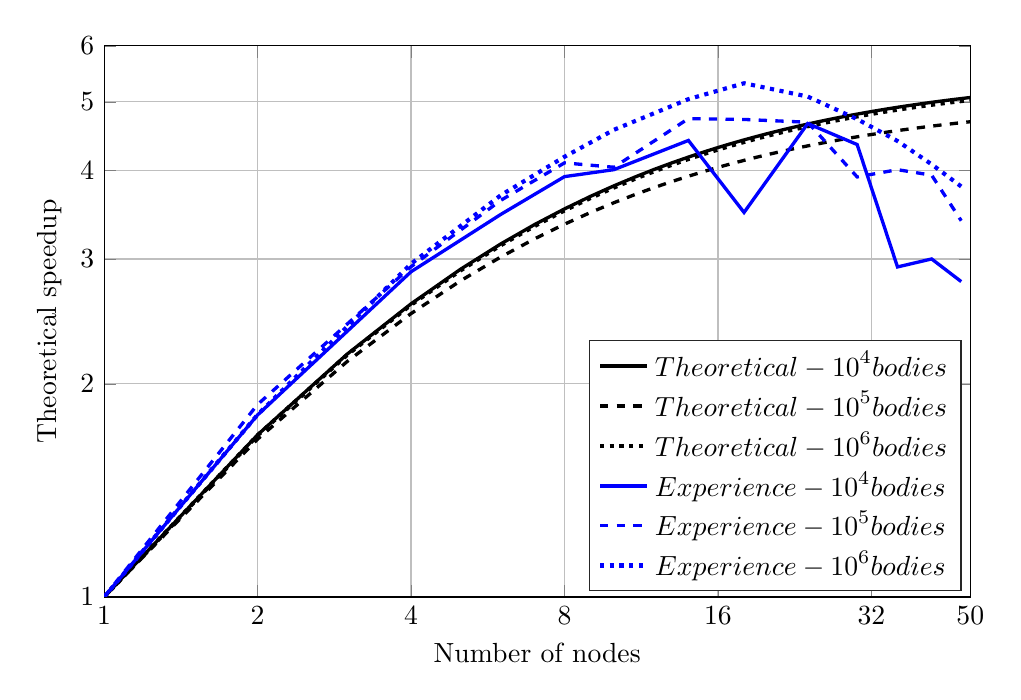
\begin{tikzpicture}

\begin{axis}[%
width=11cm,
height=7cm,
at={(0.758333in,0.48125in)},
scale only axis,
xmode=log,
xmin=1,
xmax=50,
xtick={1,2,4, 8, 16, 32, 50},
xticklabels={{1},{2},{4},{8},{16},{32}, {50}},
xminorticks=true,
xlabel={Number of nodes},
xmajorgrids,
xminorgrids,
ymode=log,
ymin=1,
ymax=6,
ytick={1,2,3,4,5,6},
yticklabels={{1},{2},{3},{4},{5},{6}},
yminorticks=true,
ylabel={Theoretical speedup},
ymajorgrids,
yminorgrids,
legend style={at={(0.99,0.01)},anchor=south east,legend cell align=left,align=left,draw=white!15!black}
]
\addplot [color=black,solid,line width=1.2pt]
  table[row sep=crcr]{%
1	1\\
2	1.6937899510075\\
3	2.20334216965291\\
4	2.59344192354659\\
5	2.90168652023547\\
6	3.15139327484974\\
7	3.3577912616699\\
8	3.53124848721009\\
9	3.67906809928399\\
10	3.80654294649019\\
11	3.91760274810478\\
12	4.01522637737897\\
13	4.10171304425647\\
14	4.17886567627005\\
15	4.24811796544492\\
16	4.31062428772729\\
17	4.36732456528899\\
18	4.41899185637153\\
19	4.46626781077842\\
20	4.50968945352666\\
21	4.54970967422904\\
22	4.58671308287264\\
23	4.62102841010838\\
24	4.6529382998322\\
25	4.68268711217689\\
26	4.71048719307112\\
27	4.73652395078827\\
28	4.76095999619283\\
29	4.7839385421459\\
30	4.80558621224844\\
31	4.8260153752877\\
32	4.84532609626958\\
33	4.86360777554752\\
34	4.88094053271128\\
35	4.89739638043212\\
36	4.91304022454\\
37	4.92793071962079\\
38	4.94212100391271\\
39	4.95565933291098\\
40	4.96858962760298\\
41	4.98095195045862\\
42	4.9927829200442\\
43	5.00411607329853\\
44	5.01498218302057\\
45	5.02540953689811\\
46	5.03542418340513\\
47	5.0450501490685\\
48	5.05430963091904\\
49	5.06322316737192\\
50	5.07180979030545\\
};
\addlegendentry{$\text{Theoretical - 10}^\text{4}\text{ bodies}$};

\addplot [color=black,dashed,line width=1.2pt]
  table[row sep=crcr]{%
1	1\\
2	1.67045595392877\\
3	2.15122262669296\\
4	2.51282529355071\\
5	2.7946831136722\\
6	3.0205556205969\\
7	3.2056163683254\\
8	3.36000997234063\\
9	3.49077610601366\\
10	3.60295297064327\\
11	3.70024139831853\\
12	3.78542098544317\\
13	3.86061994924348\\
14	3.92749537556431\\
15	3.98735675224598\\
16	4.04125256988969\\
17	4.09003226056965\\
18	4.13439129697756\\
19	4.17490456175802\\
20	4.21205139842249\\
21	4.24623466659004\\
22	4.27779541150231\\
23	4.30702428195494\\
24	4.33417050754315\\
25	4.35944902295441\\
26	4.38304617067176\\
27	4.40512430237917\\
28	4.42582551945939\\
29	4.44527473482025\\
30	4.46358219549278\\
31	4.48084557363471\\
32	4.49715170969999\\
33	4.5125780734583\\
34	4.52719399474528\\
35	4.541061705201\\
36	4.55423722401665\\
37	4.5667711142776\\
38	4.57870913143453\\
39	4.59009278143526\\
40	4.60095980286681\\
41	4.61134458491023\\
42	4.62127853086129\\
43	4.63079037531225\\
44	4.63990646174279\\
45	4.64865098616808\\
46	4.6570462115893\\
47	4.6651126572488\\
48	4.67286926607704\\
49	4.68033355320799\\
50	4.68752173801374\\
};
\addlegendentry{$\text{Theoretical - 10}^\text{5}\text{ bodies}$};

\addplot [color=black,dotted,line width=1.5pt]
  table[row sep=crcr]{%
1	1\\
2	1.691421267001\\
3	2.19800335525537\\
4	2.58512724431123\\
5	2.89059086663529\\
6	3.1377672908751\\
7	3.34188660133655\\
8	3.51329796445007\\
9	3.65927987990264\\
10	3.78510039650046\\
11	3.89466642690251\\
12	3.9909366804081\\
13	4.07619286756916\\
14	4.15222285768443\\
15	4.22044742612696\\
16	4.28200987107316\\
17	4.33784059917366\\
18	4.38870447407415\\
19	4.4352360663391\\
20	4.4779662641571\\
21	4.51734261811561\\
22	4.55374507636363\\
23	4.58749828431542\\
24	4.61888129324529\\
25	4.64813529300237\\
26	4.67546982260366\\
27	4.70106779715546\\
28	4.72508960619414\\
29	4.74767647758651\\
30	4.76895325608716\\
31	4.78903071203335\\
32	4.80800747033416\\
33	4.82597163066769\\
34	4.84300213505739\\
35	4.85916992761708\\
36	4.87453894240263\\
37	4.88916694837746\\
38	4.90310627503627\\
39	4.91640443789987\\
40	4.92910467963817\\
41	4.94124643980696\\
42	4.95286576394922\\
43	4.96399566100014\\
44	4.97466641645997\\
45	4.98490586759234\\
46	4.99473964591353\\
47	5.00419139142041\\
48	5.01328294232639\\
49	5.02203450351125\\
50	5.03046479641954\\
};
\addlegendentry{$\text{Theoretical - 10}^\text{6}\text{ bodies}$};

\addplot [color=blue,solid,line width=1.2pt]
  table[row sep=crcr]{%
1	1\\
2	1.80713496852145\\
4	2.87873543044448\\
6	3.46853470902353\\
8	3.92262444207154\\
10	4.01145474426364\\
14	4.41106854023671\\
18	3.49046119963774\\
24	4.66022547019529\\
30	4.35277619408911\\
36	2.92403879940567\\
42	3.00083166872478\\
48	2.78813677860674\\
};
\addlegendentry{$\text{Experience - 10}^\text{4}\text{ bodies}$};

\addplot [color=blue,dashed,line width=1.2pt]
  table[row sep=crcr]{%
1	1\\
2	1.8695639507855\\
4	2.92631062444475\\
6	3.63149384737242\\
8	4.10094373594427\\
10	4.04283600141889\\
14	4.73510091840613\\
18	4.72262035762503\\
24	4.67998551474486\\
30	3.91772658535315\\
36	4.01121144765421\\
42	3.9405887654349\\
48	3.39801052272871\\
};
\addlegendentry{$\text{Experience - 10}^\text{5}\text{ bodies}$};

\addplot [color=blue,dotted,line width=1.5pt]
  table[row sep=crcr];
\node[draw=black,fill=white, anchor=west] at (2,7.2) {Barnes-Hut};
}
\end{tikzpicture}
\end{frame}

\begin{frame}{Weak Scaling}
\begin{tikzpicture}[overlay,remember picture,shift={(current page.south west)}]
%\grille
\only<1>{
\node[anchor=south west] at (0,0) {% This file was created by matlab2tikz.
% Minimal pgfplots version: 1.3
%
%The latest updates can be retrieved from
%  http://www.mathworks.com/matlabcentral/fileexchange/22022-matlab2tikz
%where you can also make suggestions and rate matlab2tikz.
%
\begin{tikzpicture}

\begin{axis}[%
width=10.7cm,
height=3cm,
at={(0.758333in,1.37cm)},
scale only axis,
xmode=log,
xmin=1,
xmax=8,
xminorticks=true,
xlabel={Number of nodes},
xmajorgrids,
xminorgrids,
xtick={1, 2, 3, 4, 5, 6, 7, 8},
xticklabels={{1},{2},{3},{4},{5},{6},{7},{8}},
ymin=0,
ymax=1,
ylabel={Efficiency},
ymajorgrids,
legend style={legend cell align=left,align=left,draw=white!15!black}
]
\addplot [color=blue,solid,line width=1.2pt]
  table[row sep=crcr]{%
1	1\\
2	0.756022222489609\\
3	0.476306460007734\\
4	0.344895238110588\\
5	0.17231894047816\\
6	0.0981318273010437\\
7	0.0643015717878828\\
8	0.0536375400360533\\
};
\addlegendentry{$\text{BF - 10}^\text{4}\text{ bodies per node}$};

\addplot [color=blue,dashed,line width=1.2pt]
  table[row sep=crcr]{%
1	1\\
2	0.637555427058201\\
3	0.343172333025313\\
4	0.208015206665949\\
5	0.132620712503118\\
6	0.095214562576354\\
7	0.0699260175960599\\
8	0.0541372092748112\\
};
\addlegendentry{$\text{BF - 10}^\text{5}\text{ bodies per node}$};

\end{axis}

\begin{axis}[%
width=10.7cm,
height=3cm,
at={(0.758333in,5.37cm)},
scale only axis,
xmode=log,
xmin=1,
xmax=8,
xminorticks=true,
xlabel={Number of nodes},
xtick={1,2,3, 4, 5, 6, 7, 8},
xticklabels={{1},{2},{3},{4},{5},{6},{7},{8}},
xmajorgrids,
xminorgrids,
ymode=log,
ymin=1,
ymax=10000,
yminorticks=true,
ylabel={Running time [s]},
ymajorgrids,
yminorgrids
]
\addplot [color=blue,solid,line width=1.2pt,forget plot]
  table[row sep=crcr]{%
1	1.25145425759091\\
2	1.65531411691818\\
3	2.62741399218182\\
4	3.62850546863636\\
5	7.26243008527273\\
6	12.7527866545455\\
7	19.4622654282727\\
8	23.3316862919091\\
};
\addplot [color=blue,dashed,line width=1.2pt,forget plot]
  table[row sep=crcr];
}
\only<2>{
\node[anchor=south west] at (0,0) {% This file was created by matlab2tikz.
% Minimal pgfplots version: 1.3
%
%The latest updates can be retrieved from
%  http://www.mathworks.com/matlabcentral/fileexchange/22022-matlab2tikz
%where you can also make suggestions and rate matlab2tikz.
%
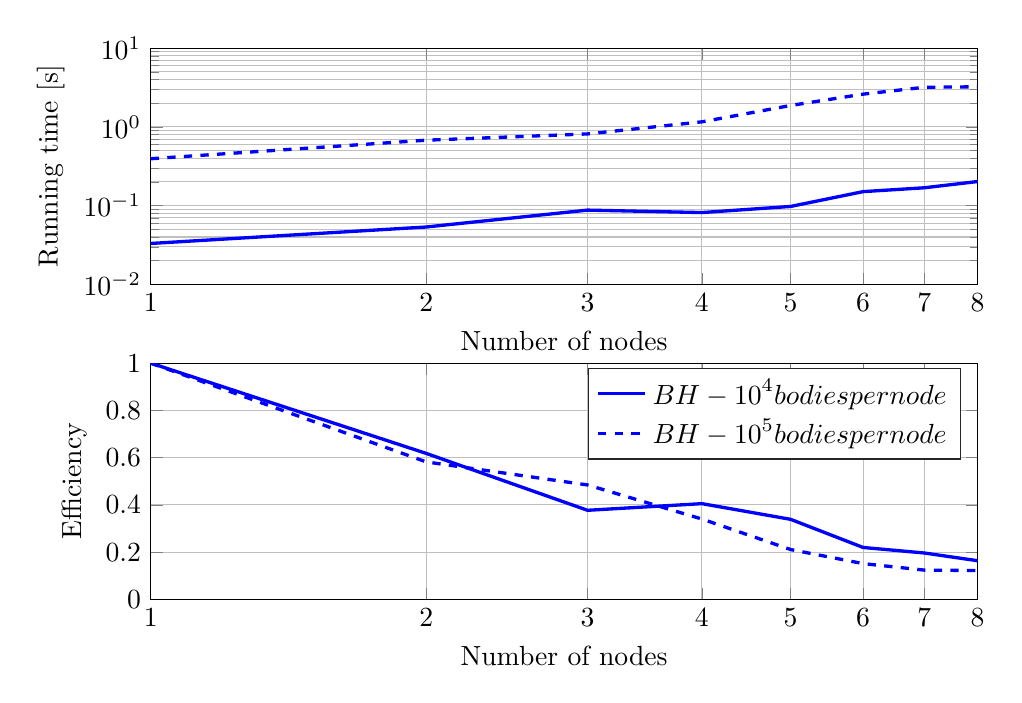
\begin{tikzpicture}

\begin{axis}[%
width=10.5cm,
height=3cm,
at={(0.758333in,5.37cm)},
scale only axis,
xmode=log,
xmin=1,
xmax=8,
xminorticks=true,
xlabel={Number of nodes},
xmajorgrids,
xminorgrids,
xtick={1,2,3, 4, 5, 6, 7, 8},
xticklabels={{1},{2},{3},{4},{5},{6},{7},{8}},
ymode=log,
ymin=0.01,
ymax=10,
yminorticks=true,
ylabel={Running time [s]},
ymajorgrids,
yminorgrids
]
\addplot [color=blue,solid,line width=1.2pt,forget plot]
  table[row sep=crcr]{%
1	0.03308295392\\
2	0.0535573495098039\\
3	0.0877561541372549\\
4	0.0816696460392157\\
5	0.0976765590196078\\
6	0.150651544509804\\
7	0.168636937058824\\
8	0.202365228823529\\
};
\addplot [color=blue,dashed,line width=1.2pt,forget plot]
  table[row sep=crcr]{%
1	0.394341795484314\\
2	0.677898941568627\\
3	0.814232577647059\\
4	1.15994181019608\\
5	1.87087138627451\\
6	2.60626458431373\\
7	3.18709408627451\\
8	3.23189081568628\\
};
\end{axis}

\begin{axis}[%
width=10.5cm,
height=3cm,
at={(0.758333in,1.37cm)},
scale only axis,
xmode=log,
xmin=1,
xmax=8,
xtick={1,2,3, 4, 5, 6, 7, 8},
xticklabels={{1},{2},{3},{4},{5},{6},{7},{8}},
xminorticks=true,
xlabel={Number of nodes},
xmajorgrids,
xminorgrids,
ymin=0,
ymax=1,
ylabel={Efficiency},
ymajorgrids,
legend style={legend cell align=left,align=left,draw=white!15!black}
]
\addplot [color=blue,solid,line width=1.2pt]
  table[row sep=crcr]{%
1	1\\
2	0.617710813227306\\
3	0.376987280780977\\
4	0.405082616669043\\
5	0.338699010817517\\
6	0.219599168582351\\
7	0.19617857449854\\
8	0.163481414827691\\
};
\addlegendentry{$\text{BH - 10}^\text{4}\text{ bodies per node}$};

\addplot [color=blue,dashed,line width=1.2pt]
  table[row sep=crcr];
}
\end{tikzpicture}

\end{frame}

\section{Conclusion}

\begin{frame}{Conclusion}
\onslide<1->
\bf How can we make it better?
\normalfont
\begin{itemize}
\item Use MPI I/O to write the positions of the bodies
\item Implement a heuristic for the construction of the tree \\(don't rebuild it at each iteration)
\item Use a sorting algorithm for the bodies to build the tree in parallel
\item Use RK4 (or another schema) to update the bodies
\end{itemize}
\onslide<2->
\bf What did we learn? 
\normalfont
\begin{itemize}
\item A clever algorithm in serial can be better (and more ecological) than an easy parallel algorithm.
\item Complex serial algorithm can be "easily" updated to a parallel version
\item We can always make an algorithm faster. But is it worth it?
\end{itemize}
\end{frame}

\begin{frame}[standout]
\only<1>{
{\Huge
Thank you
}
}
\only<2>{
\begin{tikzpicture}[overlay,remember picture,shift={(current page.south west)}]
%\grille
\node at (6.4, 4.5) {\href{https://www.youtube.com/embed/h0nFjeHjKYs}{\includegraphics[width=12cm,height=6.75cm]{images/title.png}}};
\end{tikzpicture}
}
\end{frame}

\end{document}